\documentclass[11pt]{article}

\usepackage{amssymb,amsmath,amsfonts,amsthm}
\usepackage{latexsym}
\usepackage{graphics}
\usepackage{indentfirst}
\usepackage{lmodern}
\usepackage[hyphens]{url}
\usepackage{hyperref}
\usepackage{mathrsfs}
\usepackage{array}
\usepackage{mathtools}
\usepackage{graphicx}
\usepackage{setspace}
\usepackage{enumerate}
\usepackage{tikz}
\usepackage{url,color}
\usepackage{xcolor}
\usepackage{chngcntr}
\usepackage{multicol}
\usepackage{comment}
\usepackage{float}
\usepackage{algpseudocode}
\usepackage{subcaption}
\usepackage[ruled]{algorithm2e}
\usepackage{booktabs}
\usepackage{caption}
\usepackage[letterpaper,margin=2cm,top=2.5cm,bottom=2.5cm]{geometry}

\AtBeginEnvironment{algorithm}{\setstretch{1.2}}

\hypersetup{colorlinks=true,citecolor=blue,linkcolor=blue,urlcolor=blue}

%%%%%%%%%%%%%%%%%%%%%%%%%%%%%%%%%%%%%%%%%%%%%%%%%%%%%%%%%%
%% Theorem environments
%%%%%%%%%%%%%%%%%%%%%%%%%%%%%%%%%%%%%%%%%%%%%%%%%%%%%%%%%%
\newtheorem{theorem}{Theorem}[section]
\newtheorem{lemma}{Lemma}[section]
\newtheorem{proposition}{Proposition}[section]
\newtheorem{corollary}{Corollary}[section]
\newtheorem{remark}{Remark}[section]
\newtheorem{definition}{Definition}[section]

%%%%%%%%%%%%%%%%%%%%%%%%%%%%%%%%%%%%%%%%%%%%%%%%%%%%%%%%%%
%% Math shorthands
%%%%%%%%%%%%%%%%%%%%%%%%%%%%%%%%%%%%%%%%%%%%%%%%%%%%%%%%%%
\newcommand{\N}{\mathbb{N}}
\newcommand{\Z}{\mathbb{Z}}
\newcommand{\E}{\mathbb{E}}
\newcommand{\R}{\mathbb{R}}
\newcommand{\norm}[1]{\left\lVert#1\right\rVert}
\newcommand{\todo}[1]{\textcolor{red}{[#1]}}

\allowdisplaybreaks

%%%%%%%%%%%%%%%%%%%%%%%%%%%%%%%%%%%%%%%%%%%%%%%%%%%%%%%%%%
%% Title, authors, abstract
%%%%%%%%%%%%%%%%%%%%%%%%%%%%%%%%%%%%%%%%%%%%%%%%%%%%%%%%%%

\title{Diffusion Proposals for Redistricting Markov Chains}

\author{Alaittin K\i rt\i \c{s}o\u{g}lu \\
        \small Department of Applied Mathematics, Illinois Institute of Technology \\
        \small Chicago, IL 60616 \\
        \small \texttt{kirtisoglu@hawk.iit.edu}}

\date{\today}

\begin{document}

\maketitle

\begin{abstract}
Recombination (ReCom) chains are the standard Markov chain Monte Carlo
tool for sampling redistricting plans, and they are routinely run under
a Metropolis filter that nominally targets a compactness-tempered
distribution. We introduce a proposal built from graph diffusion. One
convex energy on the merged pair of districts, a kernel-weighted
Laplacian smoothness term plus a fidelity term that anchors each move to
the current plan, is minimized under global population balance and
rounded at random. The diffusion view yields a small theory of the
proposal: its optimum is a single linear solve whenever balance is
slack, the expected number of units a proposal moves is an explicit
high-pass filter norm with a provable ceiling, and mobility is governed
by feasibility rather than by the Metropolis ratio, which gives a tuning
rule. Correcting the rounding with an exact Metropolis--Hastings step
gives, to our knowledge, the first optimization-based redistricting
proposal with a detailed-balance proof. Mixed with the forest-lifted
recombination move Metropolized to the same target, it yields a
reversible sampler for kernel-weighted compactness distributions,
validated against enumerated targets. On Iowa it roughly doubles the
effective samples per second of the forest move alone under perimeter
and density targets, and adds nothing on the spanning-tree-weighted
measure. The reason is structural, and we measure it: the tree move is
an independence sampler from the untempered spanning-tree measure, so
its acceptance decays exponentially with the size of the merged pair
under any compactness-tempered target, while the local move has a dial
for the same effect. On an enumerated test bed we also show, at the
level of distributions, that plain and tempered ReCom do not sample
their nominal target and sit close to the spanning-tree-weighted
measure.
\end{abstract}

%% Rebuilt 2026-10-22 after the Forest ReCom kill test and the scaling
%% experiment. Precinct-scale sections are placeholders marked \todo.

%════════════════════════════════════════════════════════════════════════════════
\section{Introduction}\label{sec:intro}
%════════════════════════════════════════════════════════════════════════════════

\subsection{The redistricting problem and ReCom's role}\label{sec:intro-problem}

Political redistricting seeks a partition of a region into districts
that are contiguous, population balanced, compact, and respectful of
communities of interest. Computational approaches model the problem
on the dual adjacency graph $G = (V,E)$ of geographic units. A valid
$k$-district plan is a partition $P = \{V_1, \ldots, V_k\}$ of $V$
with each $G[V_i]$ connected and the populations $p(V_i)$ nearly
equal; $\mathcal{P}_k(G)$ denotes the space of valid plans, and even
four districts over the 99 counties of Iowa admit roughly $10^{24}$ of
them~\cite{fifield2020essential}. Markov chain Monte Carlo is the
standard tool for sampling it. Flip chains~\cite{fifield2020automated}
mix slowly; Recombination (ReCom)~\cite{deford2021recombination}
merges two adjacent districts, draws a uniform spanning tree of the
merged subgraph and cuts a balanced edge, and is now the workhorse of
the field, with reversible~\cite{cannon2022spanning},
forest-lifted~\cite{autry2023metropolized} and
multi-scale~\cite{autry2020multiscale} extensions.

ReCom has two blind spots that this paper addresses. The first is
that the uniform spanning-tree split treats every edge of the merged
subgraph identically, so the proposal is determined by topology
alone, while shared boundary length, population density and
administrative boundaries all carry signal. County-weighted
trees~\cite{clelland2022colorado}, region-aware
surcharges~\cite{gerrychain2024} and SpecReCom~\cite{davies2025spectral}
inject some of it, but each shifts the chain's stationary distribution
in an uncharacterized way. The second blind spot is shared by the
exact versions of the tree move: they propose from one fixed law, the
spanning-tree measure on balanced splits, and whenever the target is
not close to that law the Metropolis step must undo the mismatch on
every proposal. We show that the resulting acceptance decays
exponentially in the size of the merged pair, which is the structural
reason an exact sampler for compactness targets needs a second kind
of move.

\subsection{Contribution}\label{sec:intro-contribution}

We introduce a diffusion proposal for ReCom-style MCMC and the exact
sampler built on it. The core object is one Laplacian energy on the
merged-pair subgraph $H = G[V_i \cup V_j]$,
\begin{equation}\label{eq:core-energy}
  E(x) \;=\; \alpha\, x^\top L\, x \;+\; \beta\, \|x - x_0\|^2,
  \qquad
  (1 - \varepsilon)\bar p \;\le\; p^\top x \;\le\; (1+\varepsilon)\bar p,
\end{equation}
where $L$ is the kernel-weighted Laplacian of $H$, $x_0$ encodes the
current bipartition, and the balance constraint is anchored to the
global per-district ideal. The Laplacian term counts (or weights) cut
edges; the fidelity term keeps each move local. Four contributions
follow.

\begin{enumerate}
  \item \textbf{A proposal with a theory of its own behavior}
    (\S\ref{sec:diffusion-theory}). The optimum of the energy is one
    implicit Euler step of the graph heat equation with timestep
    $\tau = \alpha/\beta$. It is a single linear solve whose output
    lies in the unit cube automatically (Lemma~\ref{lem:row-stochastic});
    under single-shot Bernoulli rounding the expected number of units
    moved is an explicit high-pass filter norm, growing like
    $2\tau$ times the pair's boundary for small $\tau$ and bounded by
    half the pair for any $\tau$ (Proposition~\ref{prop:move-size},
    Corollary~\ref{cor:small-tau}); and the chain's mobility is a
    feasibility effect with an interior optimum in $\tau$, given to
    within counting noise by a two-swap law (\S\ref{sec:mobility}).
  \item \textbf{An exactly reversible correction} (\S\ref{sec:qp-mh}).
    Correcting the rounding with an exact Metropolis--Hastings step
    yields Chain E, to our knowledge the first optimization-based
    redistricting proposal with a detailed-balance proof
    (Proposition~\ref{prop:qpmh-db}), verified to machine precision on
    an enumerated fiber and, by a batch-means test on a million-step
    run, indistinguishable from its target (\S\ref{sec:exp-2x3}).
  \item \textbf{An exact sampler for kernel-weighted compactness
    targets, and a measurement of when its local component matters}
    (\S\ref{sec:hybrid}, \S\ref{sec:exp-iowa}, \S\ref{sec:exp-scaling}).
    We lift Chain E to the spanning-forest state space and mix it with
    the forest-lifted recombination move~\cite{autry2023metropolized}
    Metropolized to an arbitrary kernel-weighted target. On Iowa,
    under a criterion fixed before the runs, the mixture gives $1.6$ to
    $2.3$ times the forest move's effective samples per second under
    perimeter and density targets on two seeds, and $0.8$ to $0.9$
    times under the spanning-tree-weighted tempered measure. The
    reason is structural: the forest move is an independence sampler
    from the untempered spanning-tree measure, its acceptance on
    $N \times N$ grids falls like $e^{-0.24 N}$ under
    compactness-tempered targets with or without tree weights, and
    the per-proposal mismatch in its Hastings ratio grows with the
    boundary length. The local move loses acceptance with pair size
    too, but has a dial for it, the move-size law; the tree move has
    none.
  \item \textbf{A ground-truth calibration of what the ReCom family
    samples} (\S\ref{sec:exp-5x5}, \S\ref{sec:exp-iowa-calib}). On a
    fully enumerated $5 \times 5$ fiber the tempered chain's cut
    distribution is 220 noise-floor standard deviations from its
    nominal target and close to the tree-weighted tempered measure,
    while the exact chain is indistinguishable from the nominal
    target; on Iowa the exact sampler puts the nominal target's mean
    cut count near $88$ and the tree-weighted measure's at $41$, where
    tempered ReCom sits at $40$.
\end{enumerate}

\paragraph{Positioning.} A deterministic optimization that sets the
parameters of a random proposal which is then corrected exactly has
ancestors outside redistricting: randomize-then-optimize
\cite{bardsley2014randomize} and Zanella's informed
proposals~\cite{zanella2020informed}, of which Chain E is an instance
on the space of plans, so our priority claim is scoped to
redistricting. Within redistricting, the known-target samplers
(Metropolized forest recombination, RevReCom, the cycle walk, the
marked edge walk, BUD~\cite{autry2023metropolized,cannon2022spanning,
deford2025cycle,mcwhorter2025marked,akitaya2026bud}) achieve
computable transition probabilities by lifting to spanning-forest
state spaces, while Chain E does so at the partition level; the two
routes are complementary and the forest move is the global component
of our sampler. Bonsai sampling~\cite{clelland2026bonsai} draws
independent plans from a specified law without a chain.

\paragraph{Roadmap.}\label{sec:intro-roadmap}
\S\ref{sec:related} reviews related work and \S\ref{sec:background}
sets up notation. \S\ref{sec:model} develops the proposal, its
theory, the exact chain, and the sampler; \S\ref{sec:experiments}
reports the calibration, the convergence validation, the kill test
against the forest move, the scaling experiment, and the Iowa
calibration. Appendices hold hyperparameters and a reproducibility
checklist.

%════════════════════════════════════════════════════════════════════════════════
\section{Related work}\label{sec:related}
%════════════════════════════════════════════════════════════════════════════════

\paragraph{MCMC for redistricting.} Flip chains~\cite{fifield2020automated}
mix poorly~\cite{najt2024empirical}; ReCom~\cite{deford2021recombination}
is standard, with multi-scale~\cite{autry2020multiscale}, forest-lifted
\cite{autry2023metropolized}, sequential Monte Carlo
\cite{mccartan2023sequential,osullivan2026generalized,cannon2024repetition},
parallel-tempering~\cite{chuang2025multiscale} and reversible
\cite{cannon2022spanning} variants. The compactness-tempered target
practitioners run under a Metropolis filter originates in Herschlag
et al.~\cite{herschlag2020quantifying}; the 50-State
Atlas~\cite{mccartan2022simulated} is the standard benchmark. The
2022--2026 literature's theme is that a sampler is only as defensible
as its target, and RevReCom, forest recombination, the cycle
walk~\cite{deford2025cycle} and the marked edge
walk~\cite{mcwhorter2025marked} all pay for computable transition
probabilities with lifted state spaces. Cannon, Pegden and
Tucker-Foltz~\cite{cannon2024sampling} give a polynomial-time sampler
for the spanning-tree measure on grids with constant $k$,
Gold~\cite{gold2026adversarial} exhibits configurations that trap
recombination for exponentially many steps, Akitaya et
al.~\cite{akitaya2022reconfiguration} prove reachability
PSPACE-complete when $k$ and the step size grow with the graph, and
mixing bounds for the chains used in practice remain open.

\paragraph{Weighted and geography-aware proposals.} County-weighted
trees~\cite{clelland2022colorado}, GerryChain's region-aware
surcharges~\cite{gerrychain2024} and Tapp's compactness-aware
split~\cite{tapp2025compactness} weight edges inside the ReCom
proposal; in all three the induced stationary distribution is
uncharacterized. What the unweighted tree proposal induces is better
understood: Clelland et al.~\cite{clelland2021compactness} measured
ReCom's sampling probability to decay roughly exponentially in cut
length, Procaccia and Tucker-Foltz~\cite{procaccia2022compact} proved
that compact plans have many spanning trees, and Tapp, Proebsting and
Ramsay~\cite{tapp2025parameter} study how tolerance and county
settings move ensembles. Our calibration (\S\ref{sec:exp-5x5}) makes
the first observation exact on an enumerated fiber, and our scaling
experiment (\S\ref{sec:exp-scaling}) turns the second into a statement
about acceptance: the exponential that makes compact plans tree-rich
is what an exact tree move pays, per proposal, to target anything
else. The known-target samplers above handle only tree-count-based
families; the gap this paper fills is a proposal that takes an
arbitrary nonnegative edge kernel as input together with an exact
accept/reject step against a stated target.

\paragraph{Optimization and spectral lines.} An operations-research
literature treats districting as exact
optimization~\cite{gurnee2021fairmandering,swamy2023multiobjective,
validi2022imposing,validi2022political,dobbs2024facilitating}, and
hybrids with sampling are emerging: short bursts~\cite{cannon2023voting}
use ReCom as an optimizer, and Brous and Shmoys~\cite{brous2025recom}
put a Gurobi integer program inside a local search. The integer form
of our energy belongs to that matheuristic line (\S\ref{sec:disc-future});
its proximal term is the quadratic analogue of local
branching~\cite{fischetti2003local}. On the spectral side,
SpecReCom~\cite{davies2025spectral} replaces the tree with a
Fiedler-vector cut of a randomly weighted Laplacian, and
diffuse-interface segmentation~\cite{chan2001active,bertozzi2012diffuse,
merkurjev2013mbo,pilavci2021graph} supplies the Laplacian-plus-fidelity
energy we use; Jacobs and Walch~\cite{jacobs2018pde,jacobs2018auction}
brought threshold dynamics to redistricting as a continuum PDE method
outside MCMC. To our knowledge this is the first use of the graph
Ginzburg--Landau lineage as a proposal inside redistricting MCMC. The
cut-edge count as a compactness measure is due to Duchin and
Tenner~\cite{duchin2018discrete}.

%════════════════════════════════════════════════════════════════════════════════
\section{Background: plans and ReCom}\label{sec:background}
%════════════════════════════════════════════════════════════════════════════════

\subsection{Dual graph and \texorpdfstring{$k$}{k}-district plans}\label{sec:background-graph}

Let $G = (V, E)$ be the dual graph of a state, with vertices
representing geographic units (precincts, census blocks, counties) and
edges encoding shared boundaries. Each vertex $v$ carries a population
$p_v \ge 0$ and may carry additional attributes (demographic vectors,
shapefile geometry). A \emph{$k$-district plan} is a partition
$P = \{V_1, \ldots, V_k\}$ of $V$ such that each induced subgraph
$G[V_i]$ is connected (\emph{contiguity}) and the populations satisfy
\begin{equation}\label{eq:pop-balance}
  (1 - \varepsilon)\bar p \;\le\; p(V_i) \;\le\; (1 + \varepsilon)\bar p,
  \qquad \bar p := \frac{p(V)}{k},
\end{equation}
for a tolerance $\varepsilon \in [0, 1)$. We write $\mathcal{P}_k(G; \varepsilon)$
for the set of valid plans. The \emph{cut edges} of a plan are
\[
  \partial P \;=\; \{(u,v) \in E : P(u) \ne P(v)\},
\]
and we call $|\partial P|$ the \emph{cut-edge count} of $P$. This
quantity is the discrete analog of the perimeter of the district
boundaries and serves as our primary compactness
metric~\cite{duchin2018discrete}. For a nonnegative edge kernel $w$ we
write $w(\partial P) = \sum_{e \in \partial P} w_e$ for the
\emph{weighted cut}.


\subsection{Recombination (ReCom)}\label{sec:background-recom}

Recombination~\cite{deford2021recombination} is a Markov chain on
$\mathcal{P}_k(G; \varepsilon)$. One step selects two adjacent
districts $V_i, V_j$, forms $H = G[V_i \cup V_j]$, draws a uniform
spanning tree of $H$ by Wilson's algorithm~\cite{wilson1996generating},
searches its edges for one whose removal leaves two
$\varepsilon$-balanced components (redrawing the tree if none exists),
and replaces $V_i, V_j$ by the two components. Many units move at
once and contiguity is automatic, which is the advantage over flip
chains.

\textbf{Chains compared.} Table~\ref{tab:chains} lists the chains of
this paper.

\begin{table}[htbp]
\centering
\footnotesize
\begin{tabular}{llll}
\toprule
Chain & Method & Mechanism & Stationarity claim \\
\midrule
V & Vanilla ReCom~\cite{deford2021recombination} & spanning-tree split, always accept & unknown target \\
A & Tempered ReCom & ReCom + MH on cuts (symmetric-$q$) & approximate \\
E & QP-MH (this work, \S\ref{sec:qp-mh}) & QP + Bernoulli rounding + exact MH & \textbf{exact} \\
T & Partition-level tree move (\S\ref{sec:tree-partition}) & uniform tree, uniform edge, tree-count MH & \textbf{exact} \\
F & Forest move (\S\ref{sec:forest}) & forest-lifted ReCom, balanced edge, exact MH & \textbf{exact} \\
H & Hybrid (this work, \S\ref{sec:hybrid}) & mixture of F and lifted E, any kernel-weighted target & \textbf{exact} \\
\bottomrule
\end{tabular}
\caption{The chains compared. Chains E, T, F and H carry exact
  Metropolis--Hastings corrections; Chain A relies on the
  symmetric-$q$ approximation (\S\ref{sec:qp-mh}) and Chain V has no
  stated target. Chain T explains Chain A; Chain F is the baseline the
  sampler is judged against.}
\label{tab:chains}
\end{table}

Tempered ReCom uses a Metropolis--Hastings filter targeting
$\pi(P) \propto \exp(-\lambda |\partial P|)$ with the symmetric-$q$
approximation, which treats forward and reverse proposal
probabilities as equal, at the locked-in $\lambda = 0.10$ of
Appendix~\ref{app:hyperparams}. All chains enforce the global
two-sided balance window of Equation~\eqref{eq:balance-window} on
every move; we note (\S\ref{sec:exp-balance}) that the raw GerryChain
\texttt{recom} proposal alone does not.

%════════════════════════════════════════════════════════════════════════════════
\section{The QP-diffusion model, its theory, and the sampler}\label{sec:model}
%════════════════════════════════════════════════════════════════════════════════

\subsection{Locality kernels}\label{sec:kernels}

Choosing the edge weights $w_{ij}$ is the most important modeling
decision. The kernel determines what \emph{smoothness} means and
therefore controls how district boundaries move under the relaxation.
We restrict all weights to geographic neighbors,
\begin{equation}\label{eq:kernel-local}
  w_{ij} = 0 \quad \text{if } (v_i, v_j) \notin E,
\end{equation}
ensuring that diffusion operates only through geographic adjacency and
preventing long-range interactions that could produce disconnected
districts.

\paragraph{Uniform kernel ($k_{\mathrm{unif}}$).} $w_{ij} = 1$ for
every edge. The Laplacian $L$ is the combinatorial graph Laplacian;
$x^\top L x$ is exactly the cut edge count. In the $\beta \to 0^+$
limit the proposal approaches a balanced Fiedler-style split.

\paragraph{Perimeter kernel ($k_{\mathrm{perim}}$).} $w_{ij} = |\partial v_i \cap \partial v_j|$
(shared-boundary length). The Laplacian quadratic form $x^\top L x$
is then the \emph{geographic perimeter} of the partition, weighted by
boundary segment length. This kernel discourages fragmented districts
and favors boundaries that cut along short segments.

\paragraph{Density kernel ($k_{\mathrm{dens}}$).} Let $\rho_v$ denote
the population density at vertex $v$ (population per unit area). A
Gaussian density kernel
\[
  w_{ij} \;=\; |\partial v_i \cap \partial v_j| \cdot
  \exp\!\Bigl( -\frac{(\rho_i - \rho_j)^2}{\sigma^2} \Bigr)
\]
encourages cuts along sharp density gradients (urban--rural
boundaries) while preserving the topological role of shared boundary
length.

\paragraph{Demographic kernel ($k_{\mathrm{demog}}$).} A Gaussian
similarity kernel on a vector of attributes $d_v$ encourages
communities of interest. We define it for completeness and do not use
it: a kernel built on race would make race the predominant districting
criterion, which the \emph{Shaw v.\ Reno} line of cases subjects to
strict scrutiny, so any such use needs legal review and is more
defensible for attributes that are legitimate factors in the
jurisdiction. Nonnegative linear combinations of kernels remain
valid.

\subsection{The convex QP}\label{sec:qp-model}

Let $H = G[V_i \cup V_j]$ be the merged subgraph of two adjacent
districts. Let $L_H$ be the kernel-weighted Laplacian of $H$, let
$x_0 \in \{0,1\}^{|V_H|}$ encode the current bipartition (1 for
vertices in $V_i$, 0 for vertices in $V_j$), and let $p$ be the
population vector restricted to $H$. Fix weights $\alpha, \beta > 0$
and balance tolerance $\varepsilon \in (0, 1)$. Crucially, the balance
constraint is anchored to the \emph{global} per-district ideal
$\bar p = p(V)/k$ from Equation~\eqref{eq:pop-balance}, not to
$p(V_H)/2$. Both sides of the split must individually satisfy the
plan-validity bound, which yields the two-sided window
\begin{equation}\label{eq:balance-window}
  \ell \;=\; \max\bigl((1-\varepsilon)\bar p,\; p(V_H) - (1+\varepsilon)\bar p\bigr),
  \qquad
  u \;=\; \min\bigl((1+\varepsilon)\bar p,\; p(V_H) - (1-\varepsilon)\bar p\bigr).
\end{equation}
Anchoring to $p(V_H)/2$ instead (a tempting simplification, and one
present in an earlier version of our own implementation) only bounds
the local split. Because $p(V_H)$ itself drifts as the chain moves
population between pairs, district populations can ratchet outside the
global tolerance by a factor of up to $(1+\varepsilon)$ per move on
heterogeneous graphs. Our experiments audit the global bound at every
step (\S\ref{sec:experiments}).

\begin{definition}[Continuous QP-diffusion]\label{def:qp}
The continuous QP-diffusion bipartition of $H$ is
\begin{align}
  x^\star \;=\; \arg\min_{x \in [0,1]^{|V_H|}} \;\;
    & \alpha\, x^\top L_H\, x \;+\; \beta\, \|x - x_0\|_2^2 \label{eq:qp-obj} \\
  \text{subject to} \;\;
    & \ell \;\le\; p^\top x \;\le\; u,
    \label{eq:qp-balance}
\end{align}
with $\ell, u$ as in Equation~\eqref{eq:balance-window}.
\end{definition}

The first term in~\eqref{eq:qp-obj} is the kernel-weighted Laplacian
smoothness energy. For binary $x$ it equals the weighted cut count
$\sum_{(u,v) \in E(H)} w_{uv}\,\mathbf{1}[x_u \ne x_v]$, and the
continuous relaxation $x \in [0,1]^{|V_H|}$ extends this to a smooth
objective on the unit cube. The second term is the \emph{fidelity term},
which penalizes deviation from the current bipartition and ensures
that each proposed move is local. The balance constraint enforces
$\varepsilon$-balance on the proposed split.

\begin{proposition}[Convexity and well-posedness]\label{prop:convex}
The objective in~\eqref{eq:qp-obj} is strictly convex on
$[0,1]^{|V_H|}$ (since $\beta > 0$ and $L_H$ is positive semidefinite).
The feasible region defined by~\eqref{eq:qp-balance} is a nonempty
polytope whenever the current plan is valid (it then contains $x_0$).
Hence the QP admits a unique minimizer $x^\star$, computable in
polynomial time by any convex QP solver.
\end{proposition}

\paragraph{Spectral interpretation.} Projecting the interior optimality
condition $(\alpha L_H + \beta I) x^\star = \beta x_0$ onto the
eigenbasis $\{\phi_k\}$ of $L_H$ with eigenvalues
$0 = \lambda_1 \le \lambda_2 \le \cdots \le \lambda_n$ yields the
closed-form frequency response
\begin{equation}\label{eq:freq-response}
  \hat x^\star_k \;=\; \frac{\beta}{\alpha \lambda_k + \beta}\,
  \hat x_{0,k},
  \qquad \hat y_k := \phi_k^\top y.
\end{equation}
The QP therefore acts as a low-pass spectral filter on the prior $x_0$,
with cutoff controlled by the ratio $\alpha / \beta$. Equivalently, with
$\tau := \alpha / \beta$, the optimum satisfies
$(x^\star - x_0)/\tau = -L_H x^\star$, the implicit Euler
discretization of the graph heat equation $\dot x = -L_H x$. Inspecting the leading eigenvectors is a sanity check on the kernel:
noise rather than coherent regions means an uninformative kernel.

\subsection{Theory of the diffusion proposal}\label{sec:diffusion-theory}

The spectral identity is usually read as interpretation. Worked
through, it predicts how the proposal behaves, and every prediction
below is checked against the solver. Write $\tau := \alpha/\beta$ for
the diffusion timestep, $L = L_H$ for the kernel-weighted Laplacian of
the merged pair, $n = |V_H|$, and $\mathbf{1}_i \in \{0,1\}^{n}$ for
the indicator of $V_i$, so that $x_0 = \mathbf{1}_i$.

\begin{lemma}[The box constraints never bind]\label{lem:row-stochastic}
For any nonnegative kernel and any $\tau > 0$, the matrix
$(I + \tau L)^{-1}$ is symmetric, entrywise nonnegative, and has unit
row sums. Hence the unconstrained minimizer
$x^\star = (I + \tau L)^{-1} x_0$ of \eqref{eq:qp-obj} is a convex
combination of the entries of $x_0$ and lies in $[0,1]^{n}$, and the
QP of Definition~\ref{def:qp} reduces to this single linear solve
whenever the balance constraint \eqref{eq:qp-balance} is slack at
$x^\star$.
\end{lemma}

\begin{proof}
$I + \tau L$ is symmetric with positive diagonal, nonpositive
off-diagonal entries, and row sums equal to one, so it is strictly
diagonally dominant, hence a nonsingular M-matrix, and its inverse is
entrywise nonnegative. Since $L\mathbf{1} = 0$ we have
$(I + \tau L)\mathbf{1} = \mathbf{1}$ and so
$(I + \tau L)^{-1}\mathbf{1} = \mathbf{1}$. Each row of the inverse is
therefore a probability vector and $x^\star_v$ is a weighted average of
entries of $x_0 \in \{0,1\}^n$. The objective is strictly convex, so if
the unconstrained minimizer satisfies the one remaining constraint it
is the constrained minimizer.
\end{proof}

\begin{proposition}[Expected move size]\label{prop:move-size}
Under the single-shot Bernoulli rounding of \S\ref{sec:qp-mh}, and
whenever the balance constraint is slack, the expected number of units
of $H$ that a proposal reassigns is
\begin{equation}\label{eq:move-size}
  \E[\#\mathrm{flips}]
  \;=\; \|x^\star - x_0\|_1
  \;=\; 2\,\mathbf{1}_i^{\top}(I + \tau L)^{-1}\mathbf{1}_j
  \;=\; \frac{2\,|V_i|\,|V_j|}{n}
        \;-\; 2\sum_{k \ge 2}\frac{(\phi_k^{\top}\mathbf{1}_i)^2}{1 + \tau\lambda_k},
\end{equation}
where $(\lambda_k, \phi_k)$ are the eigenpairs of $L$ with
$\lambda_1 = 0$.
\end{proposition}

\begin{proof}
A unit with $x_{0,v} = 0$ flips with probability $x^\star_v$ and one
with $x_{0,v} = 1$ with probability $1 - x^\star_v$; both equal
$|x^\star_v - x_{0,v}|$ because $x^\star_v \in [0,1]$ by
Lemma~\ref{lem:row-stochastic}, which gives the first equality.
Write $P = (I + \tau L)^{-1}$. For $v \in V_i$,
$1 - x^\star_v = \sum_{u \in V_j} P_{vu}$ by unit row sums, and for
$v \in V_j$, $x^\star_v = \sum_{u \in V_i} P_{vu}$; summing and using
symmetry of $P$ gives $2\,\mathbf{1}_i^{\top} P\, \mathbf{1}_j$.
Expanding $P = \sum_k \phi_k\phi_k^{\top}/(1 + \tau\lambda_k)$ with
$\phi_1 = \mathbf{1}/\sqrt{n}$ gives the $k = 1$ term
$|V_i||V_j|/n$, and since $\phi_k \perp \mathbf{1}$ for $k \ge 2$,
$\phi_k^{\top}\mathbf{1}_j = -\phi_k^{\top}\mathbf{1}_i$, which
gives the sum. Clipping at $\delta = 10^{-12}$ changes the expectation
by at most $\delta n$.
\end{proof}

\begin{corollary}[Small-timestep law, monotonicity, and ceiling]\label{cor:small-tau}
Let $|\partial_w(V_i, V_j)|$ be the boundary of the pair measured in
the proposal's kernel. Then $\E[\#\mathrm{flips}]$ is increasing in
$\tau$,
\[
  \E[\#\mathrm{flips}] \;=\; 2\tau\,|\partial_w(V_i,V_j)| + O(\tau^2)
  \quad (\tau \to 0),
  \qquad
  \E[\#\mathrm{flips}] \;\le\; \frac{2\,|V_i|\,|V_j|}{n}
  \quad\text{for every } \tau,
\]
with equality in the limit $\tau \to \infty$. For a balanced pair the
ceiling is $n/2$, half the merged pair.
\end{corollary}

\begin{proof}
Each subtracted term in \eqref{eq:move-size} is nonnegative and
decreasing in $\tau$, which gives monotonicity and the bound, and the
terms vanish as $\tau \to \infty$. For the small-$\tau$ law, expand
$(1 + \tau\lambda_k)^{-1} = 1 - \tau\lambda_k + O(\tau^2)$; the
$\tau^0$ terms cancel because
$\sum_{k \ge 2}(\phi_k^{\top}\mathbf{1}_i)^2 = |V_i| - |V_i|^2/n =
|V_i||V_j|/n$, and the $\tau^1$ term is
$2\tau\sum_k \lambda_k(\phi_k^{\top}\mathbf{1}_i)^2 =
2\tau\,\mathbf{1}_i^{\top}L\,\mathbf{1}_i = 2\tau|\partial_w|$.
\end{proof}

Three consequences follow. The continuous proposal is far cheaper
than ``solve a QP'' suggests, since it is one linear solve in the
common case. The move size is a design dial with a known scale, so to
propose moves of about $m$ units one sets
$\alpha/\beta \approx m / (2|\partial_w|)$ while the small-timestep law
holds; \S\ref{sec:exp-scaling} uses this dial. And the dial has a hard
stop. No choice of $\alpha$ and $\beta$ can lift the expected move
above half the merged pair, so mobility cannot be bought by tuning,
which is the structural reason a global move is needed alongside the
exact local chain (\S\ref{sec:mobility}, \S\ref{sec:hybrid}). The
kernel enters through $|\partial_w|$, so a perimeter kernel takes
larger steps exactly where the geographic border is long.

\begin{figure}[htbp]
  \centering
  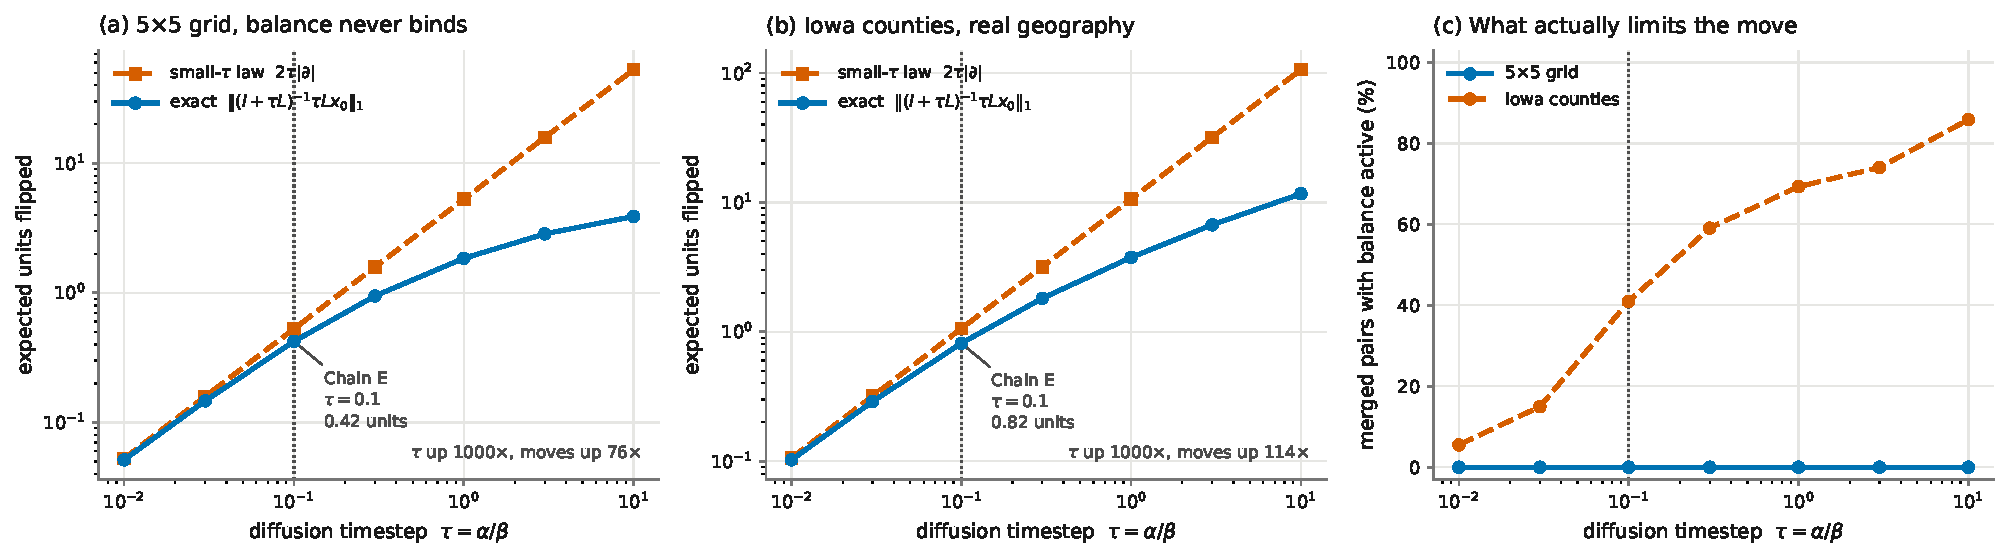
\includegraphics[width=\textwidth]{fig/spectral_move_size.pdf}
  \caption{The move-size law against the solver. (a)~On the enumerated
    $5 \times 5$ fiber, 1\,411 merged pairs drawn from 200 plans; the
    exact filter norm of \eqref{eq:move-size} and the small-timestep
    law $2\tau|\partial_w|$ agree for $\tau \le 0.03$ and separate as
    the gain saturates. Raising $\tau$ by $1000\times$ raises the move
    by $76\times$, and the last decade buys $2.1\times$. The locked
    Chain E setting $\tau = 0.1$ is marked. (b)~The same on Iowa, 127
    pairs from 25 tree-partition plans. (c)~Fraction of merged pairs
    whose balance constraint is active. On the uniform grid it never
    is, so the proposal is a linear solve at every step; on real county
    geography it is active for 41\% of pairs at $\tau = 0.1$ and 86\%
    at $\tau = 10$, so there the population constraint, not the
    diffusion, caps the move.}
  \label{fig:spectral-move-size}
\end{figure}

\textbf{Verification.} Across 10\,766 linear solves the unconstrained
optimum never left the unit cube; on 120 pairs with balance slack,
Gurobi's solution and the linear solve agree to $1.1 \times 10^{-4}$.
The small-timestep law's median relative error is $2.5\%$ at
$\tau = 0.01$, $7.4\%$ at $0.03$ and $24\%$ at $0.1$
(Figure~\ref{fig:spectral-move-size}). At the locked setting the
expected move is $0.42$ units on the $5 \times 5$ fiber and about one
unit on Iowa, which is the quantitative content of Chain E's
stickiness.

\subsection{Deterministic rounding, and why it blocks the correction}\label{sec:rounding}

The continuous optimum $x^\star \in [0,1]^{|V_H|}$ must be rounded to
a bipartition. The natural deterministic choice is a Cheeger
sweep~\cite{chung1997spectral}: sort the entries, scan the thresholds,
keep the balanced connected candidate with the smallest cut. As a
proposal it has a defect no repair fixes: an argmin-plus-sweep map is
deterministic, so the reverse proposal has zero probability and the
Hastings ratio degenerates. A chain built on it is a heuristic with no
stationarity claim. The same defect is why the forest move of
\S\ref{sec:forest} keeps the tree draw and the cut-edge draw random
rather than optimized.

\subsection{The exactly reversible QP-MH chain (Chain E)}\label{sec:qp-mh}

Replacing the deterministic rounding of \S\ref{sec:rounding} with
\emph{single-shot randomized rounding} restores a tractable,
everywhere-positive proposal density and yields an exactly reversible
chain. One step of Chain E is as follows.

\begin{enumerate}
  \item Pick an adjacent district pair $(V_i, V_j)$ uniformly at random
    from the $|\mathrm{bp}(P)|$ boundary pairs of the current plan $P$;
  \item Solve the (deterministic) QP of Definition~\ref{def:qp} on
    $H$ for $x^\star \in [0,1]^{|V_H|}$;
  \item Draw the proposal $x' \in \{0,1\}^{|V_H|}$ by independent
    Bernoulli rounding from the \emph{clipped} optimum,
    $x'_v \sim \mathrm{Bern}\bigl(\mathrm{clip}(x^\star_v;
    \delta, 1-\delta)\bigr)$ with $\delta = 10^{-12}$,
    \emph{once}, with no retry on infeasibility. Clipping is part of
    the proposal: the optimum can have coordinates exactly $0$ or $1$,
    and sampling from the same clipped vector whose density enters
    the acceptance ratio gives every binary $x'$ positive
    probability;
  \item Accept with probability
    \begin{equation}\label{eq:qpmh-accept}
      \min\Bigl(1,\;
      \frac{\pi(P')}{\pi(P)}\,
      \frac{q(x_0 \mid P', \{i,j\})}{q(x' \mid P, \{i,j\})}\,
      \frac{|\mathrm{bp}(P)|}{|\mathrm{bp}(P')|}\Bigr),
    \end{equation}
    where $q(\cdot \mid P, \{i,j\})$ is the Bernoulli product density
    induced by the QP optimum at the corresponding state, and proposals
    that violate contiguity or the balance
    window~\eqref{eq:balance-window} are rejected outright.
\end{enumerate}

Here $\pi$ is any target on plans; the paper uses
$\pi_w(P) \propto \exp(-\lambda\, w(\partial P))$ for a kernel $w$,
which reduces to the tempered cut-count target for the uniform
kernel, and in \S\ref{sec:hybrid} also the tree-weighted variant.

\begin{proposition}[Detailed balance of Chain E]\label{prop:qpmh-db}
Chain E satisfies detailed balance with respect to any target $\pi$ on
$\mathcal{P}_k(G; \varepsilon)$ that is positive on valid plans.
\end{proposition}

\begin{proof}
Fix the deterministic kernel $w$ and write $\Omega$ for the space of
valid plans, taken as \emph{labeled} assignments so that a Bernoulli
draw and its complement are distinct states and the proposal map is a
bijection; $\pi$ is label-invariant, so forgetting labels after
sampling recovers the unlabeled law. For distinct $P, P' \in \Omega$,
a step changes only the two selected districts, so if $P$ and $P'$
differ on more than two districts, or on two whose union $H$ is
disconnected and hence never selected, then $K(P,P') = K(P',P) = 0$.
Otherwise the differing pair $\{i,j\}$ is the unique pair that can
generate either move, and it is adjacent in both plans because every
bipartition of the connected graph $H$ into nonempty parts is crossed
by an edge. Three facts make the transition probability explicit.
First, the feasible set $\{x \in [0,1]^{V_H} : \ell \le p^\top x \le u\}$
of the QP depends on $(H, \varepsilon, \bar p)$ only, not on the
endpoint, and contains both $x_0(P)$ and $x_0(P')$ because the global
window~\eqref{eq:balance-window} is exactly the validity condition of
the two sides. This is where globality is essential: a window anchored
to the merged-pair half $(1 \pm \varepsilon)\,p(V_H)/2$ lets a valid
plan fail its own pair's window, zeroing a reverse density whose
forward counterpart is positive. Second, the objective has Hessian
$2(\alpha L_H + \beta I) \succ 0$, so the optimum is unique and a
deterministic function of the endpoint and the pair. Third, clipping
before sampling puts every Bernoulli factor in $[\delta, 1-\delta]$, so
every binary labeling of $V_H$ has probability at least
$\delta^{|V_H|} > 0$, and because the rounding is single-shot the
density $q_{\to} = q(x_0(P') \mid P, \{i,j\})$ is the exact probability
that the proposal from $P$ equals $P'$: no feasibility
renormalization, whose state-dependent constant would not cancel,
enters. Hence
\[
  \pi(P)\, K(P, P') \;=\;
  \frac{\pi(P)\, q_{\to}}{|\mathrm{bp}(P)|}\,
  \min\Bigl(1,\;
  \frac{\pi(P')\, q_{\gets}\, |\mathrm{bp}(P)|}
       {\pi(P)\, q_{\to}\, |\mathrm{bp}(P')|}\Bigr)
  \;=\;
  \min\Bigl(
  \frac{\pi(P)\, q_{\to}}{|\mathrm{bp}(P)|},\;
  \frac{\pi(P')\, q_{\gets}}{|\mathrm{bp}(P')|}
  \Bigr),
\]
which is symmetric in $(P, q_{\to}) \leftrightarrow (P', q_{\gets})$.
Draws that leave a side empty, disconnected or outside the window
land on states of zero target mass and are rejected with probability
one, contributing only to the diagonal; a solver failure suppresses
the forward and reverse moves identically because the solve is the
same deterministic function at both endpoints. Detailed balance and
stationarity follow~\cite{tierney1998note}.
\end{proof}

\begin{remark}[Verification and ergodicity]\label{rem:qpmh-scope}
The proof treats the solve as exact; the implementation is
deterministic (fixed kernel, no jitter, sorted pair enumeration),
which is what the argument uses. We assembled the full transition
kernel of the implementation on the enumerated $2 \times 3$ grid
($k = 2$, $\varepsilon = 1/3$, 18 labeled valid states) and verified
$\pi(P)K(P,P') = \pi(P')K(P',P)$ entrywise to a maximum relative
violation of $1.5 \times 10^{-15}$. Detailed balance gives
stationarity, not ergodicity: within a pair every relabeling has
positive probability, but irreducibility of Chain E across pairs on
general $(G, k, \varepsilon)$ is not established, and the principled
route to global mobility is the mixture of \S\ref{sec:hybrid}.
\end{remark}

Chain E trades mobility for exactness: a proposal must be feasible in
a single Bernoulli draw and Corollary~\ref{cor:small-tau} caps its
reach, so the chain is a strictly local sampler
(\S\ref{sec:mobility}), and we present it as the local component.
Mixing it with a global kernel preserves $\pi$ only if that kernel is
also $\pi$-invariant; RevReCom is reversible for its spanning-tree
measure, not for an arbitrary $\pi$, so the construction of
\S\ref{sec:hybrid} Metropolizes the tree move toward $\pi$ using its
computable Hastings ratio~\cite{cannon2022spanning,autry2023metropolized}.

\paragraph{On the tempered baseline (Chain A).} Tempered ReCom applies
$\min(1, \exp(-\lambda \Delta|\partial P|))$ over the ReCom proposal,
which assumes a symmetric proposal. ReCom's is not: the true Hastings
ratio involves spanning-tree counts of the affected
districts~\cite{autry2023metropolized,cannon2022spanning}, so Chain A
targets $\pi$ only approximately; \S\ref{sec:exp-longrun} quantifies
the bias, and we keep the baseline because it is what practitioners
run.

\subsection{Mobility of the exact chain: feasibility, not acceptance}\label{sec:mobility}

Proposition~\ref{prop:move-size} says how far a proposal reaches.
Mobility is that reach times the probability the proposal is kept,
and the second factor has two causes of different kinds. A Bernoulli
draw can produce a split that is disconnected or outside the balance
window, in which case it is rejected with probability one before any
coin is flipped. Or it can be a valid plan that loses the Metropolis
coin. We measured both on the enumerated $5 \times 5$ fiber, with
$\alpha = \tau$ and $\beta = 1$, over 3\,000 steps per timestep from
the same initial plan (Table~\ref{tab:mobility}).

\begin{table}[htbp]
\centering
\small
\setlength{\tabcolsep}{4pt}
\begin{tabular}{rrrrrrrr}
\toprule
$\tau$ & $\E[\#\mathrm{flips}]$ & single-flip share & feasible $\mid$ single
  & $\Pr[\text{feasible}]$ & accept $\mid$ feasible & units moved / step & states \\
\midrule
0.01 & 0.036 & 0.035 & 0.000 & 0.964 & 1.000 & 0.0000 & 1 \\
0.03 & 0.126 & 0.110 & 0.000 & 0.884 & 1.000 & 0.0033 & 6 \\
0.10 & 0.385 & 0.268 & 0.000 & 0.683 & 0.999 & 0.0093 & 12 \\
0.30 & 0.909 & 0.349 & 0.000 & 0.437 & 0.989 & \textbf{0.0353} & \textbf{38} \\
1.00 & 1.914 & 0.254 & 0.000 & 0.193 & 0.983 & 0.0313 & 37 \\
3.00 & 2.672 & 0.168 & 0.000 & 0.074 & 0.986 & 0.0187 & 19 \\
\bottomrule
\end{tabular}
\caption{Chain E against the diffusion timestep on the $5 \times 5$
  fiber ($k = 5$, exact balance). ``Feasible $\mid$ single'' is the
  feasibility rate of single-unit proposals, ``accept $\mid$
  feasible'' the Metropolis acceptance rate among feasible
  proposals, and ``units moved / step'' the product of acceptance and
  accepted move size, the quantity a tuning rule should maximize.
  ``States'' counts distinct fiber states reached in 3\,000 steps.
  The locked setting of Appendix~\ref{app:hyperparams} is
  $\tau = 0.10$.}\label{tab:mobility}
\end{table}

Three facts follow. First, every single-unit proposal is infeasible at
every timestep, exactly as exact balance requires, since reassigning
one cell produces districts of sizes 4 and 6. The leading-order move
of the diffusion proposal is therefore always rejected on this fiber,
and the chain moves only through second-order coordinated draws. This
is the mechanism behind the coverage figures of \S\ref{sec:exp-5x5},
derived rather than observed. Second, the Metropolis ratio is never
the bottleneck. Given a feasible proposal, acceptance is between 98
and 100 percent throughout. The chain's stickiness is a feasibility
effect, and the natural phrase ``large moves are rarely accepted'' is
wrong in an instructive way. They are rarely feasible, and when
feasible they are accepted. Third, acceptance rate is a misleading
diagnostic for this chain. At $\tau = 0.01$ it is 96 percent while
the chain never leaves its initial state, because 96 percent of
proposals flip nothing. We report units moved per step instead.

Units moved per step has an interior maximum near $\tau = 0.3$. The
setting locked in Appendix~\ref{app:hyperparams}, $\tau = 0.1$, sits
about $3.8\times$ below it, so on this fiber the chain can be improved
for free; \S\ref{sec:exp-hybrid} shows the optimum does not transfer
to Iowa, where the balance window binds more often at larger $\tau$,
and \S\ref{sec:exp-scaling} shows that on large pairs the dial has to
be turned the other way. Even at the optimum a thousand steps move
about 35 units, and Corollary~\ref{cor:small-tau} says no timestep can
lift the per-proposal reach above half the merged pair. Both
statements matter. Chain E can be several times more mobile than
shown, and several times is not enough, which is why a global move is
required (\S\ref{sec:hybrid}). Under a loose tolerance single flips
become feasible and mobility gains a first-order term in $\tau$, which
is why the same chain climbs steadily on Iowa
(\S\ref{sec:exp-iowa-calib}) while freezing on the exact-balance grid.

\textbf{The mobility law.} On an exact-balance fiber the cheapest
feasible draw is a swap, one unit $u \in V_i$ and one unit $v \in V_j$
changing sides together, which preserves both populations. Rounding
flips units independently with probabilities
$p_v = |x^\star_v - x_{0,v}|$, so the probability that exactly
$\{u,v\}$ flips is $p_u p_v \prod_{w \ne u,v}(1 - p_w)$, and the
two-swap channel contributes
\begin{equation}\label{eq:mobility-law}
  M_2 \;=\; 2 \sum_{\substack{u \in V_i,\; v \in V_j \\ \text{swap feasible}}}
  p_u\, p_v \prod_{w \ne u,v} (1 - p_w)\;\alpha(u,v)
\end{equation}
units per step, where the sum runs over cross-boundary pairs whose
swap keeps both districts connected and $\alpha(u,v)$ is the
Metropolis probability of that swap, each of which costs one reverse
linear solve. For small $\tau$, $p_v = \tau b_v + O(\tau^2)$ with
$b_v$ the kernel weight of $v$'s cross-boundary edges, so
$M_2 = 2\tau^2 S_2 + O(\tau^3)$ with
$S_2 = \sum_{\text{feasible swaps}} b_u b_v$, a coefficient computable
from the current plan. We checked the law by running Chain E for
$20\,000$ steps per timestep and evaluating \eqref{eq:mobility-law}
at every step for the pair chosen and the plan visited: measured
units per step $0.0021$, $0.0105$ and $0.0320$ at $\tau = 0.03$,
$0.1$ and $0.3$ against $M_2 = 0.0018$, $0.0105$ and $0.0326$.


The two-swap channel accounts for the mobility at every timestep,
four-unit draws contribute nothing measurable even at $\tau = 0.3$,
and without the Metropolis factor the channel overpredicts by about
$20\%$. The small-timestep form $2\tau^2 S_2$ holds only for
$\tau \lesssim 0.03$. Under a loose tolerance single flips become
feasible and the law gains a first-order channel.

\subsection{Exact tree moves, the lifted local move, and the reversible hybrid}\label{sec:hybrid}

Corollary~\ref{cor:small-tau} says the local chain cannot be made
mobile by tuning, so a global move is needed, and \S\ref{sec:qp-mh}
says that move must be reversible for the same target. This
subsection gives two exact tree moves, the one we use and the one
that explains Chain A, lifts Chain E to the state space of the first,
and states the sampler. It ends with the fact that organizes the
experiments: an exact tree move proposes from one fixed law, and pays
for every target that differs from it.

\subsubsection{The partition-level tree move (Chain T)}\label{sec:tree-partition}

Pick an adjacent pair $\{i,j\}$ uniformly from $\mathrm{bp}(P)$, draw
a uniform spanning tree $T$ of $H = G[V_i \cup V_j]$ by Wilson's
algorithm, and pick one edge of $T$ uniformly among \emph{all}
$|V_H| - 1$ tree edges. If the two components $A, B$ both lie in the
window~\eqref{eq:balance-window}, assign the labels $i, j$ to them by
a fair coin and propose; otherwise reject. Every spanning tree of $H$
that yields $\{A, B\}$ on removal of one edge is a spanning tree of
$G[A]$, a spanning tree of $G[B]$, and one crossing edge, so
\[
  q(P \to P') \;=\;
  \frac{\tau(A)\,\tau(B)\,|\partial(A,B)|}
       {2\,|\mathrm{bp}(P)|\,\tau(H)\,(|V_H| - 1)},
\]
where $\tau(\cdot)$ is the spanning-tree count by the Matrix--Tree
theorem and $|\partial(A,B)|$ the number of edges between $A$ and $B$.
The reverse move shares $H$, so $\tau(H)$ and $|V_H| - 1$ cancel and
the move is accepted with probability
\[
  \min\Bigl(1,\;
  \frac{\pi(P')}{\pi(P)}\;
  \frac{\tau(V_i)\,\tau(V_j)\,|\partial(V_i,V_j)|}
       {\tau(A)\,\tau(B)\,|\partial(A,B)|}\;
  \frac{|\mathrm{bp}(P)|}{|\mathrm{bp}(P')|}\Bigr),
\]
computable from four determinants and two edge counts; the fair coin
makes the move a bijection on labeled plans. The cut edge is drawn
among all tree edges rather than among balanced ones, which is the
point: GerryChain's \texttt{recom} draws among balanced edges, which
multiplies the density by a tree-dependent normalization that does
not cancel at the partition level, and that is why Chain A is only
approximately correct. The price is acceptance, about $7\%$ on the
exact-balance $5 \times 5$ fiber and $1\%$ on Iowa, so this move is
not what practice runs and is kept here as a reference.

\subsubsection{The forest move (Chain F)}\label{sec:forest}

Recovering balanced-edge selection with an exact density means
lifting the state to a spanning forest, as Metropolized forest
recombination does~\cite{autry2023metropolized}. A labeled forest is
$\mathcal{F} = (P, \{T_d\})$, where $T_d$ is a spanning tree of
$G[V_d]$ for every district. The fiber over a plan $P$ has
$\tau(P) = \prod_d \tau(V_d)$ forests, and the lifted target
\begin{equation}\label{eq:lifted-target}
  \tilde\pi(\mathcal{F}) \;=\; \frac{\pi(P(\mathcal{F}))}{\tau(P(\mathcal{F}))}
\end{equation}
has marginal $\pi$ on plans. Every statistic we report is a function
of the plan, so traces are comparable with the partition-level
chains.

\textbf{One step.} Pick $\{i,j\}$ uniformly from $\mathrm{bp}(P)$ and
draw a uniform spanning tree $T$ of $H$. Let $B(T)$ be the set of
edges of $T$ whose removal leaves both components inside the
window~\eqref{eq:balance-window}. If $B(T)$ is empty, draw again, up
to $M$ times, then reject. Otherwise pick $e \in B(T)$ uniformly, let
$\{A, B\}$ be the components, and assign the labels by a fair coin. A
forest $\mathcal{F}' = (\ldots, T_A, T_B, \ldots)$ is reached from
exactly those draws $(\hat T, \hat e)$ with $\hat T = T_A \cup T_B \cup f$
for a crossing edge $f \in \partial(A,B)$ and $\hat e = f$, so
\begin{equation}\label{eq:forest-q}
  q(\mathcal{F} \to \mathcal{F}') \;=\;
  \frac{c_H}{2\,|\mathrm{bp}(P)|\,\tau(H)}\; S(T_A, T_B),
  \qquad
  S(T_A, T_B) \;=\; \sum_{f \in \partial(A,B)} \frac{1}{|B(T_A \cup T_B \cup f)|},
\end{equation}
where $c_H = (1 - (1 - p_H)^M)/p_H$ accounts for the retry, $p_H$
being the probability that a uniform spanning tree of $H$ has a
balanced edge. The retry is exact because $p_H$ depends on $H$ and
the window only, never on the endpoint, and the reverse move shares
$H$, so $c_H$ and $\tau(H)$ cancel. (This is not true of the local
move's rounding, whose feasibility event depends on the QP optimum at
the endpoint; that is why Chain E must be single-shot.) The Hastings
ratio is
\begin{equation}\label{eq:forest-ratio}
  \frac{\pi(P')}{\pi(P)}\;\cdot\;
  \frac{\tau(V_i)\,\tau(V_j)}{\tau(A)\,\tau(B)}\;\cdot\;
  \frac{S(T_i, T_j)}{S(T_A, T_B)}\;\cdot\;
  \frac{|\mathrm{bp}(P)|}{|\mathrm{bp}(P')|},
\end{equation}
where the tree-count ratio is the lifted target's, not the
proposal's. Each $S$ is a sum over the crossing edges of an $O(n)$
subtree-population pass, and the two determinants of the current
districts are cached, so a step costs two determinants plus
$O(|\partial|\, n)$. Our implementation differs from Autry et al.\ in
one convention: the adjacent pair is drawn uniformly from boundary
pairs, as in every other move of this paper, rather than by a uniform
cut edge; both are exact and the ratio carries the corresponding
factor.

\textbf{Two targets.} Besides $\pi_w$ we also use the tree-weighted
version $\pi_w^{\mathrm{tree}}(P) \propto \tau(P)\, e^{-\lambda\, w(\partial P)}$,
the measure that \S\ref{sec:exp-5x5} identifies as close to what
tempered ReCom samples. Under $\pi_w^{\mathrm{tree}}$ the tree-count
ratio in \eqref{eq:forest-ratio} cancels against the same factor in
$\pi(P')/\pi(P)$. Both targets are handled by the same code path; the
local move's acceptance under the tree-weighted target acquires the
tree-count ratio instead, since it changes the plan and hence
$\tau(P)$.

\subsubsection{The lifted local move and the hybrid (Chain H)}\label{sec:lifted-local}

Run Chain E on the plan against the chosen target. If it accepts,
redraw the trees of the two changed districts uniformly by Wilson's
algorithm; otherwise keep the forest. With $K_E$ $\pi$-reversible on
plans, the lifted kernel is
$\tilde K(\mathcal{F}, \mathcal{F}') = K_E(P, P') / (\tau(A)\tau(B))$,
and $\tilde\pi(\mathcal{F})\tilde K(\mathcal{F}, \mathcal{F}')$ is
symmetric because $\tau(P) = \tau(V_i)\tau(V_j)$ times the other
districts' counts, which the move does not change. Where the balance
window is slack the local solve is the linear solve of
Lemma~\ref{lem:row-stochastic}, which we use in place of the QP
solver; both paths are deterministic functions of the state and pair,
which is all Proposition~\ref{prop:qpmh-db} requires.

The hybrid takes a lifted local step with probability
$p_{\mathrm{loc}}$ and a forest step otherwise. Both kernels are
$\tilde\pi$-reversible, so the mixture is, and its marginal on plans
is $\pi$.

\begin{proposition}[Ergodicity of the hybrid]\label{prop:ergodic}
If the forest move is irreducible on the lifted space (which holds
under the standard assumptions for recombination moves;
see~\cite{deford2021recombination,cannon2024irreducibility,autry2023metropolized}),
then the mixture with the lifted local move at any
$p_{\mathrm{loc}} \in (0, 1)$ is ergodic.
\end{proposition}

\begin{proof}
Write $K = (1 - p_{\mathrm{loc}}) K_{\mathrm{F}} + p_{\mathrm{loc}}
\tilde K_{\mathrm{E}}$. If $K_{\mathrm{F}}^{t}(\mathcal{F}, \mathcal{F}') > 0$
for some $t$, then
$K^{t}(\mathcal{F}, \mathcal{F}') \ge (1 - p_{\mathrm{loc}})^{t}\,
K_{\mathrm{F}}^{t}(\mathcal{F}, \mathcal{F}') > 0$, so irreducibility
of the forest move implies irreducibility of the mixture. The forest
move rejects with positive probability at every state, so
$K(\mathcal{F}, \mathcal{F}) > 0$ and the chain is aperiodic.
\end{proof}

\textbf{Verification.} On the lifted $2 \times 3$ fiber (18 labeled
plans, 30 forests) we assembled the forest kernel, the lifted local
kernel and their mixture analytically and checked detailed balance
entrywise under both targets and both kernels: the maximum relative
violation is $1.4 \times 10^{-15}$, the closed-form proposal mass
\eqref{eq:forest-q} equals the mass obtained by enumerating every
(tree, balanced edge, coin) draw to $1.8 \times 10^{-16}$, and the
partition-level chains T, E and their mixture pass the same check
(\texttt{forest\_recom.py}, \texttt{hybrid.py}).
\S\ref{sec:exp-hybrid} tests the forest move and the hybrid against
enumerated targets on 4\,006 plans.

\subsubsection{What an exact tree move pays}\label{sec:tree-pays}

Both tree moves draw the proposed split from the same law, the
spanning-tree measure on balanced bipartitions of $H$ (Chain F up to
the $S$ factor, which stays within a factor of two of one), and given
the pair the split does not depend on the current one. On a merged
pair the tree move is therefore an \emph{independence sampler}, and
its acceptance at equilibrium is governed by how far the target's
conditional on the pair sits from that law. Two terms of \eqref{eq:forest-ratio} carry the distance.
Under $\pi_w$ the tree-count ratio does: a uniform spanning tree
favors splits with many spanning trees, and by Procaccia and
Tucker-Foltz~\cite{procaccia2022compact} the logarithm of a tree
count scales with the boundary length, so at the equilibrium of a
target that is less compact than the tree measure the ratio is
typically far below one. Under $\pi_w^{\mathrm{tree}}$ that ratio
cancels and the target ratio $e^{-\lambda \Delta w(\partial)}$
carries the distance instead, which is large whenever the tempering
makes the target more compact than an untempered tree split.

We measured the terms on Iowa over 3\,000 forest proposals from a
tree-partition start under $\pi_w$ (Table~\ref{tab:decomposition}).
The tree-count term dominates, with mean logarithm $-6$ to $-10$ and
a share of $67$ to $84$ percent of feasible proposals below $e^{-2.3}$
on that term alone, while the target, $S$ and pair-count terms are
mild. At the equilibrium of the uniform target the acceptance given a
feasible tree is $0.17$; under the tree-weighted target at the same
temperature it is $0.74$, because at $\lambda$ equivalent to $0.1$
that target is close to the untempered tree measure. The scaling
experiment of \S\ref{sec:exp-scaling} then shows what happens as the
pair grows: for a compactness-tempered target, with or without tree
weights, the mismatch grows in proportion to the boundary length and
the acceptance decays exponentially in the grid side. The local move
loses acceptance with pair size as well, because its expected move
grows with the boundary (Corollary~\ref{cor:small-tau}), but it has a
dial for it, the timestep; the tree move has none, since its proposal
is the same law whatever the target.

\begin{table}[htbp]
\centering
\footnotesize
\begin{tabular}{lrrrrrrr}
\toprule
target & $\Pr[\text{balanced}]$ & acc.\ $\mid$ feas. &
 \multicolumn{4}{c}{mean of each log term} & share, $\tau$-term $< e^{-2.3}$ \\
\cmidrule(lr){4-7}
 & & & target & tree count & $S$ & bp & \\
\midrule
uniform, $\lambda = 0.10$   & 0.41 & 0.25 & $+0.63$ & $-5.93$ & $+0.47$ & $-0.01$ & 0.67 \\
perimeter, $\lambda = 0.34$ & 0.53 & 0.22 & $+0.65$ & $-5.98$ & $+0.59$ & $-0.00$ & 0.69 \\
density, $\lambda = 0.72$   & 0.41 & 0.13 & $+1.62$ & $-9.78$ & $+0.74$ & $-0.06$ & 0.84 \\
\bottomrule
\end{tabular}
\caption{The four terms of the forest move's log Hastings
  ratio~\eqref{eq:forest-ratio} on Iowa ($k = 4$,
  $\varepsilon = 0.05$) under $\pi_w$, averaged over the feasible
  proposals of 3\,000 steps from a tree-partition start, without
  retry. The tree-count ratio is the rejection; the retry raises
  $\Pr[\text{tree balanced}]$ to $0.95$ at $2.5$ times the wall clock
  and leaves accepted moves per second unchanged.}\label{tab:decomposition}
\end{table}

%════════════════════════════════════════════════════════════════════════════════
\section{Experiments}\label{sec:experiments}
%════════════════════════════════════════════════════════════════════════════════

We evaluate the chains of Table~\ref{tab:chains} on the
$5 \times 5$ grid (full enumeration, ground-truth target), the
$2 \times 3$ grid (18 states, full convergence checkable), the Iowa
county dual graph (real geography, 99 counties, $k = 4$,
$\varepsilon = 0.05$), and $N \times N$ grids with $k = 2$ for the
scaling experiment. All hyperparameters are locked in
Appendix~\ref{app:hyperparams}; raw traces, per-step balance audits,
and configuration stamps are released in the project repository.

\paragraph{Statistical protocol.} Chains are autocorrelated, so no
i.i.d.\ statistic is reported on a raw trace. Effective sample sizes
(ESS) come from Geyer's initial-positive-sequence estimator computed
by FFT and are used for cut means only; distributional tests use batch
means (\S\ref{sec:exp-2x3}), and distances to enumerated targets are
read against parametric-bootstrap noise floors at the ESS
(\S\ref{sec:exp-longrun}). Chains compared by effective samples per
second are also compared per step, and checked to sit at the same
level by quarter means and by the difference of their post-burn means
in standard errors. Each chain runs on its own seeded stream; baseline
tables report seed 42, ten-seed means of Chains V and A (seeds 42 to
51) enter the calibration, and between-seed standard deviations of
the baselines are $0.4$ cuts on Iowa and $0.1$ to $0.2$ on the
$5 \times 5$ fiber.

\paragraph{Balance audit.}\label{sec:exp-balance} Every baseline run
records at every step the maximum relative deviation of any district
population from the global ideal, and all satisfy
$\varepsilon = 0.05$ throughout (Iowa maxima 0.0498--0.0500); the
exact chains enforce the window inside each move. This is not
automatic: GerryChain's raw \texttt{recom} proposal validates only one
side of each cut, and an earlier version of our local steps anchored
balance to the merged-pair half, and either slip lets populations
drift to four times the nominal tolerance on Iowa. We recommend
per-step auditing in any harness that bypasses GerryChain's validator
pipeline.

\subsection{Ground truth on the enumerated fiber: what the family samples}\label{sec:exp-5x5}

The $5 \times 5$ partition fiber, the set of all valid plans at
$k = 5$ and exact balance, has 4\,006 partitions and was enumerated
exhaustively, so every distributional quantity is exactly computable;
at $\varepsilon = 0.05$ on unit-population cells the chains traverse
precisely this fiber. In 1\,000-step runs (seed 42, burn-in 100)
Vanilla ReCom, tempered ReCom and Chain E have mean cut counts
$17.06$, $17.02$ and $16.27$ against the exact target mean $18.56$ at
$\lambda = 0.10$, and Chain E has visited only 6 states: every chain
sits far below the target at this horizon, and exactness does not buy
mixing speed.

\textbf{The origin of the gap.} The gap quantifies the compactness
bias shared by the ReCom family, and on the fiber its origin can be
identified. By the Matrix--Tree theorem we compute for each partition
the spanning-tree-count weight $\prod_i \tau(V_i)$, the measure the
RevReCom analysis identifies as the natural target of tree-based
recombination~\cite{cannon2022spanning,autry2023metropolized}. The
tree-weighted measure has $\E[|\partial P|] = 16.88$ against Vanilla
ReCom's ten-seed mean $16.95 \pm 0.11$, and the tree-weighted tempered
measure $\prod_i \tau(V_i)\, e^{-\lambda|\partial P|}$ has $16.78$
against Chain A's $16.71 \pm 0.16$; both gaps are within one
between-seed standard deviation, and both quasi-targets sit about
$1.8$ cuts below the nominal tempered mean. A mean is a
one-dimensional summary, and the long runs compare full
distributions.

\paragraph{Long-run validation at the level of distributions.}\label{sec:exp-longrun}
We run Chain A for $2 \times 10^5$ steps and Chain E for $10^5$ steps
on the fiber (seed 42, 10\% burn-in) and compare each chain's
empirical distribution with the nominal target, the tree-weighted
measure and the tree-weighted tempered measure. Every distance is
read against a parametric-bootstrap noise floor, the same distance for
independent draws from the reference at the chain's effective sample
size, since a raw total variation on 4\,006 states is uninterpretable;
and the headline statistic is the cut-count marginal, which takes five
values and is estimated to three decimals.
Table~\ref{tab:calibration-tv} and Figure~\ref{fig:calibration} give
the result.

\begin{table}[htbp]
\centering
\small
\begin{tabular}{llrrr}
\toprule
Chain & Reference measure & TV & Floor at ESS & $z$ \\
\midrule
A ($2\times10^5$ steps, ESS 12\,312) & nominal $\pi$ & 0.629 & 0.007 & $+220$ \\
 & tree-weighted & 0.065 & 0.006 & $+22$ \\
 & tree-weighted, tempered & 0.022 & 0.006 & $+6.7$ \\
\midrule
E ($10^5$ steps, ESS 28) & nominal $\pi$ & 0.079 & 0.141 & $-1.2$ \\
 & tree-weighted & 0.493 & 0.125 & $+6.9$ \\
 & tree-weighted, tempered & 0.532 & 0.125 & $+7.5$ \\
\bottomrule
\end{tabular}
\caption{Total variation between each chain's empirical cut-count
  marginal and three reference measures on the enumerated
  $5 \times 5$ fiber, with the parametric-bootstrap noise floor at the
  chain's effective sample size and the excess in floor standard
  deviations. Chain A is far from its nominal target and close to,
  though distinguishable from, the tree-weighted tempered measure.
  Chain E is indistinguishable from the nominal target it is proved
  reversible for and far from the tree measures.}\label{tab:calibration-tv}
\end{table}

\begin{figure}[htbp]
  \centering
  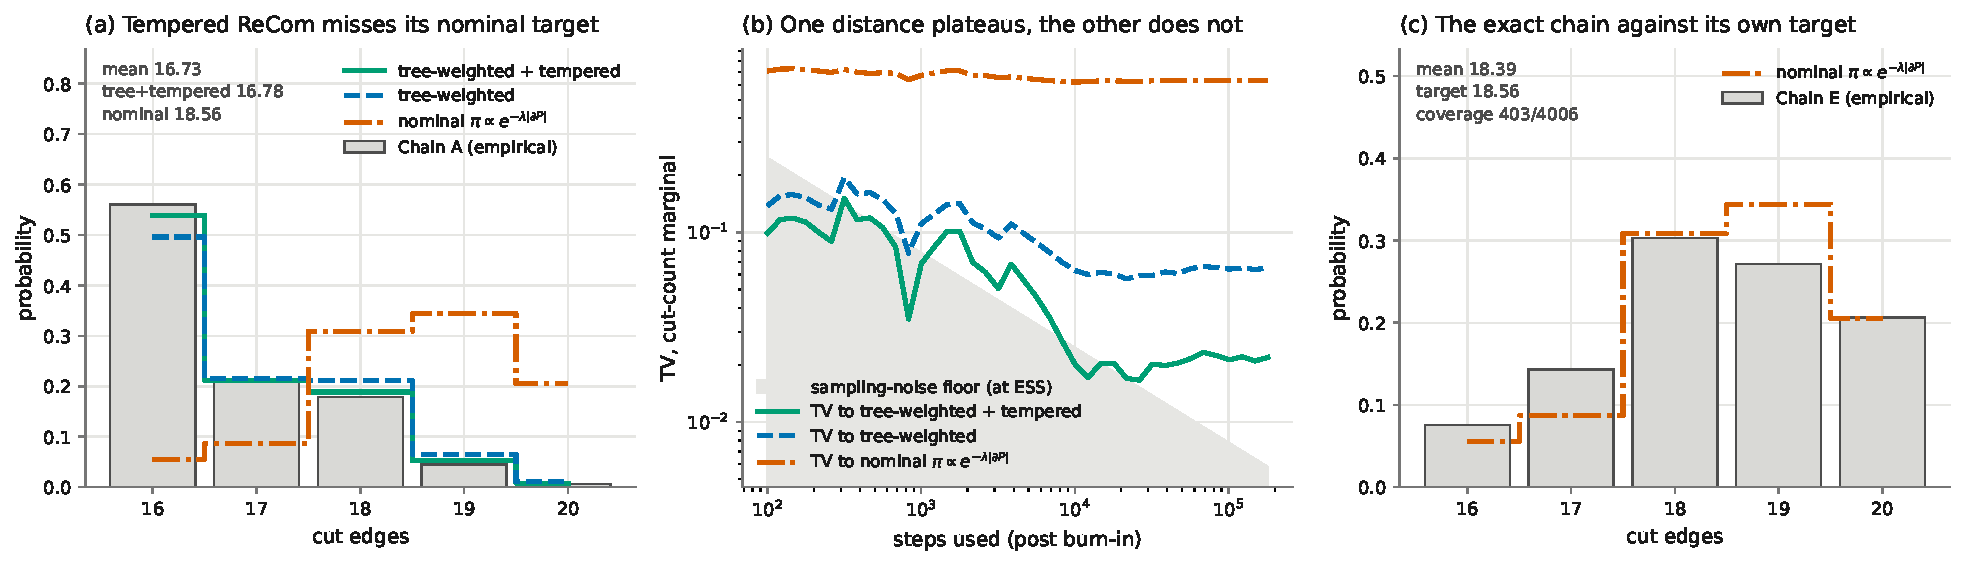
\includegraphics[width=\textwidth]{fig/calibration_5x5.pdf}
  \caption{What the chains sample. (a)~Chain A's cut-count marginal
    after $2 \times 10^5$ steps against the three reference measures.
    (b)~Total variation of the running marginal to each reference as a
    function of run length, with the noise floor at the effective
    sample size shaded; the distance to the nominal target is a
    plateau across five decades while the distance to the
    tree-weighted tempered measure descends toward the floor.
    (c)~Chain E's marginal after $10^5$ steps against its own
    target.}
  \label{fig:calibration}
\end{figure}

\emph{Chain A does not sample its nominal target, and the gap is a
plateau, not a drift.} At $2 \times 10^5$ steps the tempered chain has
visited $3\,524$ states, its mean is $16.73$, and its cut distribution
sits 220 floor standard deviations from the nominal target, at TV
$0.63$; Figure~\ref{fig:calibration}(b) shows that distance flat
across five decades of run length while the distance to the
tree-weighted tempered measure falls toward the floor. This is
convergence to a different distribution, as the symmetric-$q$ filter
predicts. The match to the tree-weighted tempered measure is close but
not exact ($6.7$ floor standard deviations at TV $0.022$), as expected
since Vanilla ReCom's stationary law is not exactly the tree measure.
\emph{Chain E samples what it states}: its cut marginal is $1.2$ floor
standard deviations from the nominal target and about $7$ from either
tree measure. Its full-state distribution converges far more slowly
(403 states visited, effective sample size 28), so that test has no
power here, and the fiber on which full convergence can be checked is
next.

\subsection{Exact convergence on the 18-state fiber}\label{sec:exp-2x3}

Detailed balance gives stationarity, not convergence, and on 4\,006
states the exact chain cannot be run to convergence in reasonable
time. On the $2 \times 3$ grid with $k = 2$ and tolerance
$\varepsilon = 1/3$, the fiber of labeled valid plans has 18 states,
the same state space on which Remark~\ref{rem:qpmh-scope} verifies
the kernel to machine precision, and a long run can cover it. We run
Chain E for $10^6$ steps (seed 42, $10\%$ burn-in, locked parameters
$\alpha = 1$, $\beta = 10$, $\lambda = 0.10$). It visits all 18
states, its acceptance rate is $0.785$, and its post-burn-in mean cut
count is $2.75992$ against the exact $2.76002$.

The distributional test uses batch means: the cut count takes two
values here, so its autocorrelation time ($17$ steps) understates that
of the 18-state occupancy process ($25$ steps), and a chi-square test
on a chain thinned by the former rejects spuriously. We split the
trace into 200 blocks of $4\,500$ steps, estimate the occupancy
covariance from the between-block scatter, and test with Hotelling's
$T^2$ on the 17 free coordinates: $F(17, 183) = 0.87$, $p = 0.61$.
Total variation to the target is $0.0110$ against a floor of about
$0.009$, down from $0.0250$ at $2 \times 10^5$ steps, the $\sqrt{n}$
rate of a converged chain. With the kernel check this is end-to-end
validation of \S\ref{sec:qp-mh}: the implemented kernel satisfies
detailed balance exactly and the chain reaches its target.

\subsection{The forest move and the hybrid against enumerated targets}\label{sec:exp-hybrid}

We run the partition-level tree move (T), the forest move (F) and
the hybrid (H, $p_{\mathrm{loc}} = 0.2$, $\tau = 0.1$) from the same
start for $2 \times 10^5$ steps on the $5 \times 5$ fiber
(Table~\ref{tab:hybrid-5x5}) against
three enumerated targets, the uniform kernel at $\lambda = 0.1$ and
at $\lambda = 1$ and a density kernel at $\lambda = 1$ built from a
synthetic central city, $\rho(x,y) = 3\exp(-r^2/2)$ with
$w_{uv} = \exp(-(\rho_u - \rho_v)^2)$, under which $\pi_w$ favors
boundaries that follow the density gradient and the tree proposal is
blind to the kernel; and then the forest move and the hybrid against
the tree-weighted versions of the same three targets. Each chain is
tested as in \S\ref{sec:exp-longrun}, by the cut-count marginal
against its noise floor and by batch-means Hotelling (cut bins of
negligible target mass merged), and we report effective samples per
second. The pre-registered criterion for the
local move is the ratio of the hybrid's effective samples per second
to the forest move's: at or above $1.5$ the local move earns its
place, below $1$ it is a passenger.

\begin{table}[htbp]
\centering
\small
\begin{tabular}{llrrrrrrr}
\toprule
Target & Chain & TV marg & $z$ & Hotel.\ $p$ & acc F & acc local & ESS/s & H/F \\
\midrule
$\pi_w$, uniform, $\lambda{=}0.1$ & F & 0.006 & $-1.2$ & 0.46 & 0.851 & --- & 211.8 & \\
 & H & 0.013 & $+0.2$ & 0.43 & 0.851 & 0.660 & 143.8 & 0.68 \\
$\pi_w$, uniform, $\lambda{=}1$ & F & 0.004 & $-1.3$ & 0.80 & 0.979 & --- & 338.6 & \\
 & H & 0.005 & $-1.3$ & 0.83 & 0.979 & 0.673 & 240.3 & 0.71 \\
$\pi_w$, density, $\lambda{=}1$ & F & 0.004 & $-1.5$ & 0.96 & 0.876 & --- & 254.5 & \\
 & H & 0.005 & $-1.5$ & 0.25 & 0.876 & 0.784 & 168.9 & 0.66 \\
$\pi_w^{\mathrm{tree}}$, uniform, $\lambda{=}0.1$ & F & 0.009 & $+0.2$ & 0.37 & 0.944 & --- & 257.3 & \\
 & H & 0.006 & $-0.8$ & 0.78 & 0.942 & 0.675 & 188.8 & 0.73 \\
$\pi_w^{\mathrm{tree}}$, uniform, $\lambda{=}1$ & F & 0.003 & $-1.0$ & 0.64 & 0.884 & --- & 265.9 & \\
 & H & 0.005 & $-0.4$ & 0.41 & 0.886 & 0.683 & 182.3 & 0.69 \\
$\pi_w^{\mathrm{tree}}$, density, $\lambda{=}1$ & F & 0.007 & $+0.1$ & 0.46 & 0.906 & --- & 259.3 & \\
 & H & 0.003 & $-1.3$ & 0.70 & 0.906 & 0.789 & 168.6 & 0.65 \\
\bottomrule
\end{tabular}
\caption{The forest move and the hybrid on the enumerated $5 \times 5$
  fiber, $2 \times 10^5$ steps each, seed 42. ``TV marg'' is total
  variation of the cut-count marginal to the enumerated target and $z$
  its excess over the noise floor at the effective sample size;
  ``Hotel.\ $p$'' is the batch-means test of \S\ref{sec:exp-2x3}; ESS
  is of the weighted-cut trace.}\label{tab:hybrid-5x5}
\end{table}

Three findings. First, every chain samples its target: all rows sit
within $1.5$ floor standard deviations of the enumerated marginal with
Hotelling $p$ between $0.25$ and $0.96$, under both target families
and both kernels, and the same holds for Chain T (within $1.8$,
$p \ge 0.21$). Second, the forest move is a different baseline from
the partition-level tree move: it accepts $0.85$ to $0.98$ against
$0.07$ and delivers $4$ to $7.5$ times the effective samples per
second on this fiber. Third, on this fiber the local move is a
passenger under every target, with ratios $0.65$ to $0.73$. That is what
\S\ref{sec:mobility} predicts under exact balance, where the local
move's first-order channel is closed, and it is also what
\S\ref{sec:tree-pays} predicts for pairs of ten cells, where the
mismatch between any of these targets and the tree measure is small.
The grid tells us the construction is right and tells us nothing yet
about where the local move matters; Iowa and the scaling experiment
do.

\subsection{The kill test on Iowa}\label{sec:exp-iowa}

On Iowa ($k = 4$, $\varepsilon = 0.05$) there is no ground truth, so
the comparison is mobility at equilibrium. We use the paper's three
kernels with $\lambda$ scaled so that $\lambda\, w(\partial P)$ at the
initial plan equals the uniform case's $0.1\,|\partial P|$, and run
the forest move alone and the hybrid at $p_{\mathrm{loc}} \in \{0.1,
0.3\}$, $\tau = 0.1$. The criterion was fixed before the long runs
were started: under $\pi_w$, with $p_{\mathrm{loc}} = 0.1$, the hybrid
passes if its effective samples per second are at least $1.5$ times
the forest move's on both the perimeter and the density target on
both seeds, with the two chains at the same level. The
$p_{\mathrm{loc}} = 0.3$ runs were added after the short runs favored
that setting and are reported as a secondary finding.

\paragraph{Short runs, direction and timing.} In $2 \times 10^5$-step
runs under $\pi_w$ the forest move accepts $0.16$ to $0.17$ and the
partition-level tree move $0.006$ to $0.012$, yet the two deliver
similar effective samples per second ($0.16$ to $0.24$ against $0.15$
to $0.40$), because a forest step costs six times more (every feasible
draw pays the determinants and the crossing-edge sums) while the
partition-level move pays them only on the one percent of draws that
balance. The hybrid beats the forest move on every kernel, by $1.4$ to
$1.8$ at $p_{\mathrm{loc}} = 0.1$ and $2.4$ to $4.4$ at $0.3$, but the
forest move's effective sample size is only $36$ to $56$ in these runs.
Under $\pi_w^{\mathrm{tree}}$ the picture inverts: the forest move
accepts $0.66$ to $0.74$, its effective sample size is about $10\,000$
per $2 \times 10^5$ steps, two hundred times its value under $\pi_w$
at the same step count, and the hybrid is a passenger at $0.86$ to
$0.93$. The per-step cost ratio of hybrid to forest move in these
single-process runs is $1.00$ at $p_{\mathrm{loc}} = 0.1$ and $0.9$ to
$1.1$ at $0.3$.

\paragraph{Long runs, the verdict.} Table~\ref{tab:iowa-long} gives
$2 \times 10^6$ steps under $\pi_w$ on two seeds, and $5 \times 10^5$
steps under $\pi_w^{\mathrm{tree}}$, where the forest move's
autocorrelation time is a hundred times shorter. Under $\pi_w$ the
pre-registered criterion passes in all four cells: ratios $1.65$ and
$2.29$ under the perimeter target, $1.95$ and $2.03$ under density,
with the two chains' means within $1.5$ standard errors in every cell
and quarter means on the same level. The forest move's effective
sample sizes are $247$ to $585$, which puts roughly $25$ percent on
each ratio, so the honest statement is ``$1.6$ to $2.3$, about two''.
At $p_{\mathrm{loc}} = 0.1$ the two chains cost the same per step on
this implementation, so the per-step ratios equal the per-second
ones. At $p_{\mathrm{loc}} = 0.3$ the ratios are $2.3$ to $4.4$; one level
check there is borderline ($z = 2.0$, density, seed 43). Under
$\pi_w^{\mathrm{tree}}$ the local move is a passenger with ratios
$0.81$ to $0.90$ at effective sample sizes of $20\,000$ to $27\,000$,
so those ratios are tight; per step the hybrid is slightly worse than
the forest move there, so a local step contributes less decorrelation
than the forest step it displaces before any cost is counted.

\begin{table}[htbp]
\centering
\footnotesize
\setlength{\tabcolsep}{4pt}
\begin{tabular}{llrrrrrrrr}
\toprule
Target & Seed & \multicolumn{2}{c}{ESS} & \multicolumn{2}{c}{ESS/s} & ratio & $z$ & \multicolumn{2}{c}{quarter means} \\
\cmidrule(lr){3-4}\cmidrule(lr){5-6}\cmidrule(lr){9-10}
 & & F & H & F & H & & & F & H \\
\midrule
\multicolumn{10}{l}{$\pi_w$, $2 \times 10^6$ steps, H at $p_{\mathrm{loc}} = 0.1$} \\
perimeter & 42 & 421 & 696 & 0.123 & 0.202 & \textbf{1.65} & $+0.2$ & 28.2 27.8 28.0 28.4 & 28.2 28.0 28.3 28.1 \\
perimeter & 43 & 247 & 572 & 0.072 & 0.165 & \textbf{2.29} & $+0.2$ & 28.6 28.2 28.7 27.9 & 28.3 28.6 28.5 28.2 \\
density & 42 & 486 & 925 & 0.177 & 0.345 & \textbf{1.95} & $-0.3$ & 18.0 18.0 18.3 17.9 & 17.9 18.0 18.2 17.9 \\
density & 43 & 585 & 1\,167 & 0.214 & 0.434 & \textbf{2.03} & $+1.5$ & 17.9 17.8 17.7 18.2 & 18.0 18.0 18.0 18.1 \\
\multicolumn{10}{l}{$\pi_w$, $2 \times 10^6$ steps, H at $p_{\mathrm{loc}} = 0.3$} \\
perimeter & 42 & 421 & 1\,116 & 0.123 & 0.324 & 2.65 & $-0.0$ & & 28.2 28.1 28.1 28.1 \\
perimeter & 43 & 247 & 1\,101 & 0.072 & 0.318 & 4.43 & $-0.9$ & & 28.2 28.3 28.2 28.1 \\
density & 42 & 486 & 1\,395 & 0.177 & 0.559 & 3.16 & $+0.8$ & & 18.1 18.2 18.1 18.1 \\
density & 43 & 585 & 1\,244 & 0.214 & 0.497 & 2.33 & $+2.0$ & & 18.0 18.1 18.0 18.2 \\
\multicolumn{10}{l}{$\pi_w^{\mathrm{tree}}$, $5 \times 10^5$ steps, H at $p_{\mathrm{loc}} = 0.1$} \\
perimeter & 42 & 27\,019 & 24\,558 & 43.9 & 37.4 & 0.85 & $-0.6$ & 13.05 13.05 13.05 13.02 & 13.03 13.04 13.02 13.05 \\
perimeter & 43 & 27\,113 & 23\,604 & 44.1 & 35.8 & 0.81 & $+0.3$ & 13.01 13.02 13.05 13.07 & 13.03 13.04 13.02 13.07 \\
density & 42 & 21\,642 & 19\,615 & 32.3 & 29.1 & 0.90 & $-1.1$ & 7.30 7.30 7.29 7.32 & 7.31 7.28 7.27 7.29 \\
density & 43 & 22\,750 & 19\,647 & 33.9 & 29.2 & 0.86 & $-1.0$ & 7.30 7.30 7.27 7.30 & 7.27 7.29 7.28 7.29 \\
\bottomrule
\end{tabular}
\caption{The Iowa kill test, long runs ($k = 4$,
  $\varepsilon = 0.05$, $\tau = 0.1$, $10\%$ burn-in). $z$ is the
  difference of the two chains' post-burn means in standard errors
  computed from their own effective sample sizes. Acceptance rates:
  forest $0.16$ (perimeter) and $0.18$ (density) under $\pi_w$,
  $0.73$ and $0.66$ under $\pi_w^{\mathrm{tree}}$; local $0.53$ and
  $0.67$ under $\pi_w$, $0.72$ and $0.84$ under
  $\pi_w^{\mathrm{tree}}$. All ten $\pi_w$ chains ran concurrently on
  one machine; cost-corrected ratios (effective samples per step
  times the single-process cost ratio of the short runs) are $1.63$,
  $2.29$, $1.99$ and $2.08$ at $p_{\mathrm{loc}} = 0.1$.}\label{tab:iowa-long}
\end{table}

\textbf{Reading.} Against the exact global move that practice runs,
the diffusion move roughly doubles effective samples per second for
geography-weighted compactness targets on Iowa and adds nothing on
the tree-weighted tempered measure at the same temperature.
\S\ref{sec:tree-pays} says why: at $\lambda$ equivalent to $0.1$ the
tree-weighted target is close to the untempered tree measure the
forest move proposes from, so there is nothing for a local move to
add, while $\pi_w$ is far from it through the tree-count term. The
next subsection shows that the second case is the general one.

\subsection{The scaling experiment}\label{sec:exp-scaling}

We run the forest move alone and the hybrid at $p_{\mathrm{loc}} = 0.3$
on $N \times N$ grids with $k = 2$, so the merged pair is the whole
graph and there is no pair-selection noise, unit populations,
tolerance $0.10$ (fixed in relative terms, so single flips are
feasible at every $N$), uniform kernel, for $N \in \{6, 8, 10, 12,
16, 20\}$ and four targets: $\pi_w$ at $\lambda = 1$ and $2$ and
$\pi_w^{\mathrm{tree}}$ at $\lambda = 0.1$ and $1$. Each chain runs
$5 \times 10^4$ steps, doubled for $N \ge 16$, from a vertical-split
start. The forest move's acceptance and the two terms of its Hastings
ratio are read from the hybrid's trace, where every forest proposal is
made from a target-distributed state even at sizes where the forest
move alone does not equilibrate within the budget.

\begin{figure}[htbp]
  \centering
  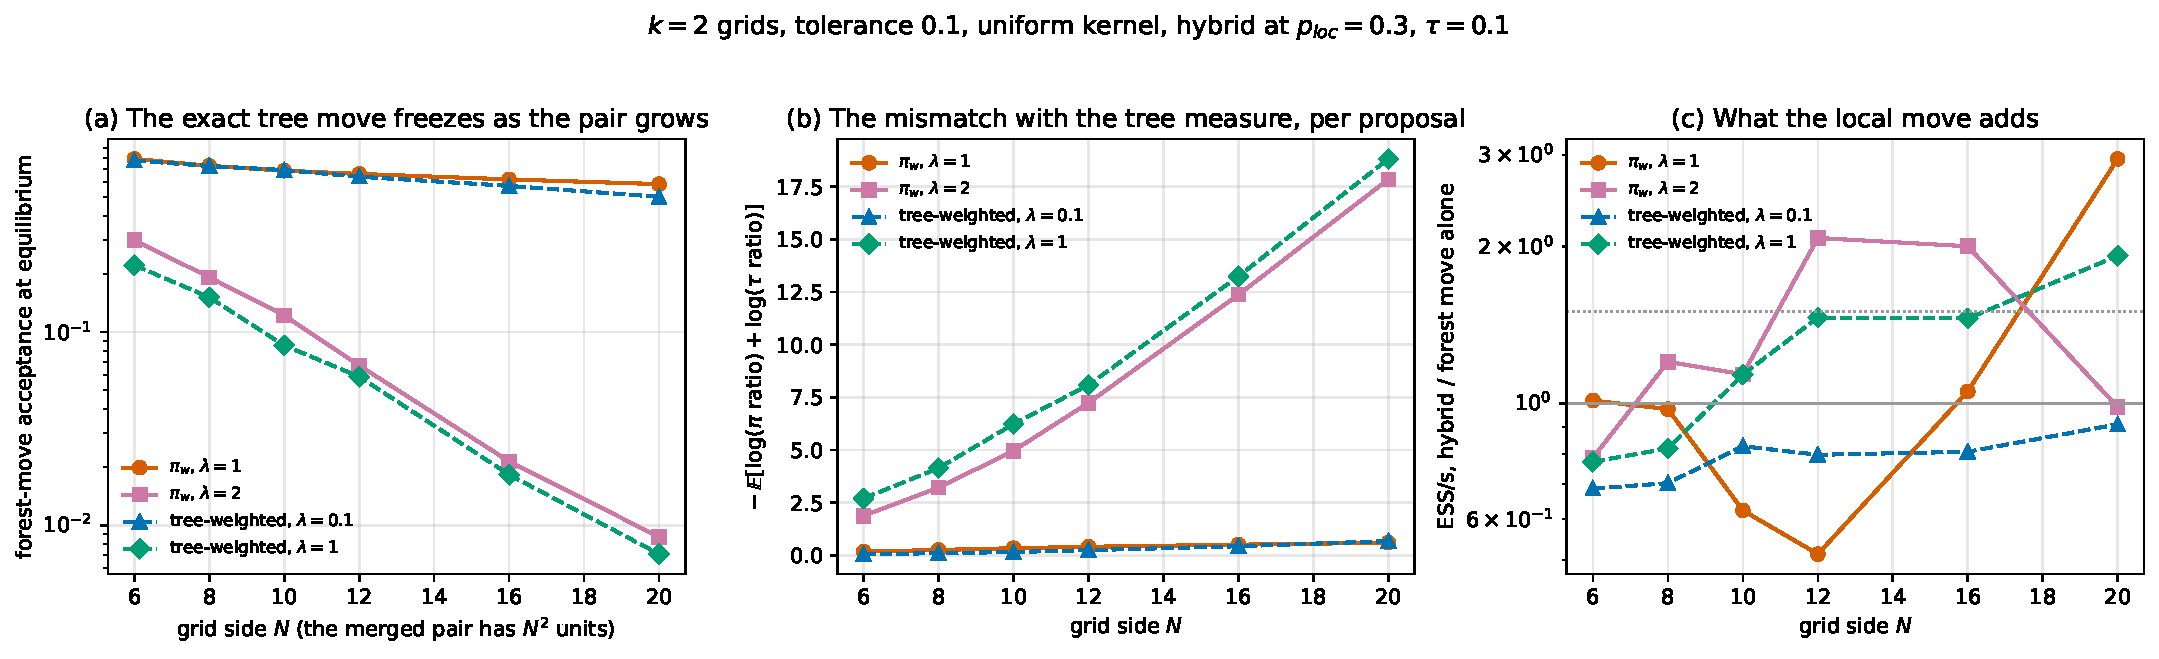
\includegraphics[width=\textwidth]{fig/forest_scaling.pdf}
  \caption{The exact tree move against grid side, $k = 2$,
    tolerance $0.1$, uniform kernel, hybrid at
    $p_{\mathrm{loc}} = 0.3$ and $\tau = 0.1$. (a)~Forest-move
    acceptance at equilibrium. (b)~Minus the mean of the target and
    tree-count log terms of \eqref{eq:forest-ratio} per feasible
    proposal, the per-proposal mismatch with the untempered tree
    measure. (c)~Effective samples per second of the hybrid over the
    forest move alone; the $N = 20$ points of the two tempered
    targets are not at equilibrium (see text).}
  \label{fig:scaling}
\end{figure}

\begin{table}[htbp]
\centering
\small
\begin{tabular}{lrrrrrr}
\toprule
 & $N = 6$ & 8 & 10 & 12 & 16 & 20 \\
\midrule
\multicolumn{7}{l}{\emph{forest-move acceptance at equilibrium}} \\
$\pi_w$, $\lambda{=}1$ & 0.79 & 0.73 & 0.69 & 0.66 & 0.62 & 0.58 \\
$\pi_w^{\mathrm{tree}}$, $\lambda{=}0.1$ & 0.78 & 0.73 & 0.69 & 0.64 & 0.57 & 0.50 \\
$\pi_w$, $\lambda{=}2$ & 0.30 & 0.19 & 0.12 & 0.067 & 0.021 & 0.009 \\
$\pi_w^{\mathrm{tree}}$, $\lambda{=}1$ & 0.22 & 0.15 & 0.085 & 0.059 & 0.018 & 0.007 \\
\multicolumn{7}{l}{\emph{mean cut length under the target}} \\
$\pi_w$, $\lambda{=}2$ & 7.2 & 10.0 & 12.6 & 15.1 & 19.8 & 25.1 \\
$\pi_w^{\mathrm{tree}}$, $\lambda{=}1$ & 6.9 & 9.7 & 12.1 & 15.0 & 20.0 & 25.1 \\
\multicolumn{7}{l}{\emph{per-proposal mismatch, $-\E[\log(\text{target ratio}) + \log(\text{tree-count ratio})]$}} \\
$\pi_w$, $\lambda{=}2$ & 1.9 & 3.2 & 5.0 & 7.2 & 12.4 & 17.9 \\
$\pi_w^{\mathrm{tree}}$, $\lambda{=}1$ & 2.7 & 4.2 & 6.2 & 8.1 & 13.2 & 18.8 \\
$\pi_w$, $\lambda{=}1$ & 0.2 & 0.3 & 0.3 & 0.4 & 0.5 & 0.6 \\
\multicolumn{7}{l}{\emph{local-move acceptance, $\tau = 0.1$ / $\tau = 0.03$}} \\
$\pi_w$, $\lambda{=}2$ & 0.39 / 0.74 & 0.32 / 0.69 & 0.25 / 0.63 & 0.19 / 0.59 & 0.12 / 0.49 & 0.08 / 0.42 \\
\multicolumn{7}{l}{\emph{ESS/s hybrid over forest, $\tau = 0.03$ (per step in parentheses)}} \\
$\pi_w$, $\lambda{=}2$ & 0.83 (0.78) & 1.03 (0.94) & 1.05 (0.91) & 1.86 (1.60) & 1.72 (1.46) & $[3.78]$ \\
$\pi_w^{\mathrm{tree}}$, $\lambda{=}1$ & 0.79 (0.76) & 0.89 (0.80) & 1.20 (1.03) & 1.53 (1.31) & 2.44 (2.11) & $[1.32]$ \\
\bottomrule
\end{tabular}
\caption{The scaling experiment. Acceptance, cut length and mismatch
  are from the hybrid's trace at $\tau = 0.1$; the local-move
  acceptance and the ratios are from the $\tau = 0.03$ rerun of the
  two tempered targets, which the move-size law calls for once the
  boundary grows. Bracketed ratios are at $N = 20$, where the forest
  move's effective sample size is $62$ and $77$ and the two chains'
  means differ by more than two standard errors, so neither chain is
  at equilibrium within the budget and the ratio is not a
  number.}\label{tab:scaling}
\end{table}

Three findings. First, the exact tree move freezes as the pair grows,
and the two tempered targets freeze it at the same rate. Under $\pi_w$
at $\lambda = 2$ and under $\pi_w^{\mathrm{tree}}$ at $\lambda = 1$
the forest move's acceptance falls on a straight line in log scale,
about $e^{-0.24 N}$, from $0.30$ and $0.22$ at $N = 6$ to $0.009$ and
$0.007$ at $N = 20$, while the per-proposal mismatch grows from about
$2$ to $19$ in proportion to the mean cut length ($7$ to $25$). The
two curves lie on top of each other in both panels of
Figure~\ref{fig:scaling}, although the tree-count term is present in
one Hastings ratio and absent from the other. What the move pays for
is the distance of the target from the untempered tree measure, not
the tree-count term as such. Under the two targets near that measure
the acceptance drifts from $0.8$ to $0.5$ over the same range and the
mismatch stays below one.

Second, the local move loses acceptance with pair size too, and has a
dial for it. At $\tau = 0.1$ its acceptance falls from $0.39$ to
$0.08$ between $N = 6$ and $20$, because its expected move
$2\tau|\partial_w|$ grows with the boundary and multi-unit draws are
more often infeasible. At $\tau = 0.03$ it is $0.74$ to $0.42$ over
the same range. The tree move has no such dial: its proposal is the
same law at every temperature and every kernel, so its acceptance is
set by the mismatch, which grows with the boundary.

Third, the local move's contribution grows with pair size where the
tree move pays. At $\tau = 0.03$ the hybrid's effective samples per
second relative to the forest move rise from below one at $N \le 10$
to $1.5$ to $2.4$ at $N = 12$ and $16$ for both tempered targets, with
the chains at the same level and the per-step ratios within $15$
percent of the per-second ones. At $N = 20$ neither chain reaches
equilibrium in $10^5$ steps under a tempered target, so that size is
beyond the budget of either chain and we do not quote a ratio. Under
the two near-proposal targets the ratio stays below one at every
size, as on Iowa under the tree-weighted target.

An exact tree move serves one family of targets well, the mildly
tempered tree measure, which is what recombination samples anyway. For
compactness targets away from it, in either direction, its acceptance
decays exponentially in the pair size, and the diffusion move, whose
reach is set by a timestep rather than by the target, is the component
that keeps an exact sampler moving. The Iowa result is one point on
these curves, at a pair size of about fifty units and a mismatch of
about six.

\subsection{Iowa: the symmetric-\texorpdfstring{$q$}{q} filter against the exact sampler}\label{sec:exp-iowa-calib}

On Iowa there is no enumeration, but the exact chains of
\S\ref{sec:hybrid} estimate both targets directly, and the forest
move reaches the equilibrium of $\pi_w$ within about a thousand steps
where the partition-level tree move needed about $10^5$. Under the
uniform kernel at $\lambda = 0.1$ the forest move and the hybrid put
the nominal target's mean cut count at $88$ to $90$ (half-run means $87.8$ to $90.1$ in the
short runs of \S\ref{sec:exp-iowa}) and the tree-weighted
tempered measure's at $41.0$ (half-run means $41.05$ and $40.93$).
Tempered ReCom with the symmetric-$q$ filter, run for 500 steps from
a tree-partition start (seed 42, burn-in 100), sits at $39.8 \pm 4.3$
cuts and Vanilla ReCom at $41.4 \pm 4.8$. On real geography the chain
practitioners run as ``targeting $\pi$'' therefore samples plans with
less than half the boundary length that $\pi$ itself has, within one
cut of the tree-weighted tempered measure, with an exact sampler on
each side of the comparison.

\subsection{Precinct scale}\label{sec:exp-precinct}

\todo{To be written. North Carolina precinct dual graph (2\,692 units,
7\,593 edges, $k = 13$, $\varepsilon = 0.05$, pairs of about 410
units), perimeter and density targets at the same tempering as Iowa,
forest move alone and hybrid at $p_{\mathrm{loc}} = 0.1$ with $\tau$
set by the move-size rule at two units per proposal
($\tau \approx 0.04$), $2 \times 10^5$ steps, two seeds with
different tree-partition starts; a timing probe first (forest step
66\,ms, local step 70\,ms in Python). Report forest acceptance, the
two Hastings terms, quarter means, ESS per step and per second, and
the ratio. Expected from \S\ref{sec:exp-scaling}: forest acceptance
falling from $0.57$ at the tree-partition start to well below
$10^{-1}$ at equilibrium, hybrid reaching equilibrium where the forest
move alone does not.}

%════════════════════════════════════════════════════════════════════════════════
\section{Discussion}\label{sec:discussion}
%════════════════════════════════════════════════════════════════════════════════

\subsection{What each chain is for}\label{sec:disc-roles}

Chain E is exact and, alone, too immobile to be a sampler; its value is
as the local component. The forest move is the mobile exact component
and the baseline practice runs; on its own measure it is hard to
improve on, and away from it its acceptance decays with pair size. The
hybrid is the practical exact sampler for kernel-weighted compactness
targets, with a small local fraction on real geography and a timestep
set by the move-size law. The partition-level tree move is the
reference whose closed form explains why Chain A is only approximate,
and Chains A and V are what practitioners run. The fidelity term is
what makes the local move local: without it the move is a fresh
spectral re-split that discards the structure the chain has found.

\subsection{Cost, and what a compiled implementation would change}\label{sec:disc-cost}

All chains here are Python. On Iowa under $\pi_w$ a forest step costs
about $1.1$\,ms, the partition-level tree move $0.18$\,ms, and a local
step about $1.5$\,ms, half of which is solver overhead on the pairs
where the balance window binds. A compiled forest step would be an
order of magnitude cheaper and the local step would gain less, so the
per-second ratios of \S\ref{sec:exp-iowa} would move against the
hybrid in Julia or Rust; this is why every comparison also reports
effective samples per step, and at $p_{\mathrm{loc}} = 0.1$ the two
coincide. Two improvements belong to a journal version: a closed-form
solve for the local move when the balance constraint is active (the
unconstrained solve shifted by a multiple of the population vector),
which removes the solver from the local step, and a per-pair timestep
$\tau = m/(2|\partial_w|)$ from Corollary~\ref{cor:small-tau} that
holds the expected move at $m$ units whatever the pair.

\subsection{Limitations}\label{sec:disc-limits}

No mixing-time bound: the scaling result is a straight line over six
grid sizes with the independence-sampler argument of
\S\ref{sec:tree-pays} as explanation, not proof. The Iowa ratios carry
about $25$ percent uncertainty and rest on two seeds; the direction,
the level agreement and the control are solid, the second decimal is
not. Chain E's irreducibility across pairs is not established, and the
hybrid inherits ergodicity from the forest move. The largest real graph
is 99 counties until \S\ref{sec:exp-precinct} is supplied.

\subsection{Future directions}\label{sec:disc-future}

The precinct-scale run and the downstream question it allows, whether
the kernel changes an ensemble's partisan statistics. The integer form
of the energy, solved as a convex mixed-integer program inside a
tempered chain, is an anchored refinement tool rather than a sampler;
an earlier version of this work found that it cut mean cut edges by
20 percent over tempered ReCom on Iowa and that simulated annealing
over ReCom proposals reached the same best plans at a fraction of the
cost, which we record so it need not be rediscovered. An informed
marked-edge selection for the marked edge
walk~\cite{mcwhorter2025marked}, with a Boltzmann draw of computable
density, would be the lifted-space analogue of Chain E. The cycle
walk~\cite{deford2025cycle} or the balanced up-down
walk~\cite{akitaya2026bud} could replace the forest move as the global
component.

%════════════════════════════════════════════════════════════════════════════════
\section{Conclusion}\label{sec:conclusion}
%════════════════════════════════════════════════════════════════════════════════

One Laplacian energy under global population balance gives a
redistricting proposal whose optimum is a linear solve, whose expected
move size is an explicit filter norm with a hard ceiling, and whose
mobility is a feasibility effect with a tuning rule. Corrected
exactly, it is Chain E, the first optimization-based redistricting
proposal with a detailed-balance proof; lifted to spanning forests and
mixed with the forest-lifted recombination move, it is a reversible
sampler for kernel-weighted compactness targets that roughly doubles
the forest move's effective samples per second on Iowa under perimeter
and density targets and adds nothing on the tree-weighted measure.
The reason is measured: an exact tree move proposes from the
untempered spanning-tree measure whatever the target, its acceptance
decays exponentially in the pair size under any compactness-tempered
target, and the local move has a dial for the same effect where the
tree move has none. On enumerated ground truth, tempered ReCom does
not sample its nominal target and sits close to the spanning-tree
measure; on Iowa the gap is a factor of two in boundary length. Kernel
choice can be a first-class decision inside the proposal and the
target, provided the induced distribution is corrected; the
spanning-tree measure is the one target a tree move samples for free;
and enumerated fibers read against noise floors are the severe test
bed a sampler should be held to.

\section*{Code and data availability}

All code, the enumerated fibers, and every artifact behind every table
and figure are in the public repository\\
\url{https://github.com/kirtisoglu/Redistricting_Diffusion_Model}\\
under \texttt{diffusion\_model/recom/}, with the scripts and command
lines listed in Appendix~\ref{app:reproducibility}. An archived
release with a persistent identifier will be deposited on acceptance.

%════════════════════════════════════════════════════════════════════════════════
\appendix
\section{Algorithm details and hyperparameters}\label{app:hyperparams}
%════════════════════════════════════════════════════════════════════════════════

\subsection{Common setup}\label{app:common}

Global two-sided balance window \eqref{eq:balance-window} on every
move, audited per step; the bare GerryChain \texttt{recom} proposal is
wrapped with a whole-plan balance check since its cut search validates
only one side. Initial plans from \texttt{recursive\_tree\_part},
redrawn until all districts satisfy the global tolerance; a vertical
split for the $k = 2$ grids. Step counts: baselines $1\,000$
($5 \times 5$) and $500$ (Iowa) with burn-in $100$; all other runs
$10\%$ burn-in, with counts as stated in the text. Seeds: base 42 with
a per-chain offset, 43 for the second Iowa long run.

\subsection{Chain-specific parameters}\label{app:chains}

Table~\ref{tab:hyperparams} lists every locked value.
\begin{table}[htbp]
\centering
\footnotesize
\begin{tabular}{lll}
\toprule
Chain & Parameter & Value \\
\midrule
A & $\lambda$ (target temperature) & 0.10 \\
E & $\alpha$, $\beta$ & 1.0, 10.0 ($\tau = \alpha/\beta = 0.1$) \\
E & Rounding & single-shot Bernoulli($x^\star$), clip $10^{-12}$ \\
T & cut edge & uniform over all tree edges; fair-coin labels \\
F & cut edge & uniform over balanced tree edges; fair-coin labels; retry up to 20 trees \\
F & pair & uniform over boundary pairs \\
H & $p_{\mathrm{loc}}$ & 0.1 (Iowa long runs), 0.1 and 0.3 (Iowa short runs), 0.2 ($5 \times 5$), 0.3 (grids) \\
H & $\tau$ & 0.1; 0.03 in the rerun of \S\ref{sec:exp-scaling} \\
Iowa $\lambda$ & uniform / perimeter / density & 0.100 / 0.343 / 0.718 (equal tempering at the start plan) \\
\bottomrule
\end{tabular}
\caption{Locked-in hyperparameters for the chains of
  Table~\ref{tab:chains}.}\label{tab:hyperparams}
\end{table}

\subsection{Compute environment}\label{app:compute}

Python 3.12 on macOS and 3.13 on Linux; Gurobi 13.0 (academic license)
for the QP solves the linear-solve path does not cover; GerryChain
0.2.22; NetworkX 3.x. One single-threaded process per chain; the ten
Iowa long runs and the scaling chains ran concurrently on an 11-core
machine, each forest chain at the same time as its hybrid partner so
that both members of a ratio see the same load, and all ratios are
also reported per step.

%════════════════════════════════════════════════════════════════════════════════
\section{Reproducibility checklist}\label{app:reproducibility}
%════════════════════════════════════════════════════════════════════════════════

\begingroup
\raggedright\sloppy
All code is under \texttt{diffusion\_model/recom/} in the repository.
Modules: \texttt{problems.py} (graphs, balanced initial plans),
\texttt{chains.py} (runners, balance-validated ReCom, per-step audit),
\texttt{qp\_model.py} (QP and QP-MH steps), \texttt{hybrid.py} (Chain T,
Chain E with the linear-solve path, their analytic check),
\texttt{forest\_recom.py} (the forest move, the lifted local move, both
targets, the analytic check on the lifted $2 \times 3$ fiber),
\texttt{kill\_stats.py} (ESS, noise floors, batch-means Hotelling).
Scripts, each writing a stamped \texttt{.npz} to
\texttt{iowa\_hybrid\_test\_out/} beside its console log:
\texttt{iowa\_target\_matched.py} (Chains V, A, E),
\texttt{long\_run\_5x5.py}, \texttt{matrix\_tree\_targets.py},
\texttt{calibration\_distance.py} and \texttt{fig\_calibration.py}
(\S\ref{sec:exp-5x5}); \texttt{db\_check\_2x3.py}, \texttt{long\_run\_2x3.py},
\texttt{gof\_2x3.py} (\S\ref{sec:qp-mh}, \S\ref{sec:exp-2x3});
\texttt{spectral\_move\_size.py}, \texttt{acceptance\_sweep.py},
\texttt{mobility\_law.py} (\S\ref{sec:diffusion-theory},
\S\ref{sec:mobility}); \texttt{forest\_validate\_5x5.py}
(Table~\ref{tab:hybrid-5x5}); \texttt{forest\_iowa.py} and
\texttt{forest\_verdict.py} (\S\ref{sec:exp-iowa});
\texttt{forest\_scaling.py} with \texttt{forest\_scaling\_parallel.py}
(\S\ref{sec:exp-scaling}); \texttt{hybrid\_validate\_5x5.py},
\texttt{hybrid\_iowa.py}, \texttt{hybrid\_iowa\_long.py} (Chain T's
rows). Command lines are in each script's docstring. The $5 \times 5$
runs and the Iowa runs under the uniform and density kernels reproduce
bit for bit from their seeds; the Iowa runs under the perimeter kernel
do not (a repeat matched for 21\,217 and 185\,390 steps and then
diverged, which we attribute to floating-point sensitivity of the QP
fallback under that kernel's wide weight range), and every
perimeter-target conclusion rests on long runs and two seeds.
\todo{Precinct scale: data file, commands and artifacts of
\S\ref{sec:exp-precinct}.}
\par
\endgroup

{\small
\bibliographystyle{plain}
\bibliography{ref}}

\end{document}
